\setcounter{chapter}{4}
\chapter{Elettrodinamica}

\section{Leggi d'induzione}

Lo studio delle trasformazioni del campo elettrostatico e del campo magnetico stazionari in sistema in moto relativo ha evidenziato che $\bold{E}$ e $\bold{B}$ sono in un qualche modo legati tra loro.

In fenomeni variabili (dipendenti dal tempo) $\bold{E}$ e $\bold{B}$ sono mutuamente accoppiati. Alcune relazioni che descrivono i campi stazionari sono incomplete e vanno estese.
Se consideriamo una carica puntiforme in moto nel sistema di riferimento del laboratorio, allora le seguenti leggi dedotte per le cariche statiche non sono pi\`u valide:
\begin{align*}
	& \bold{E} \quad \text{non \`e conservativo} \iff \nabla \times \bold{E} \neq 0 \\[0.3cm]
	& \bold{B} \quad \text{non soddisfa la legge di Amp\`ere } \iff \nabla \times \bold{B} \neq \mu_0 \bold{J}
\end{align*}
Iniziamo l'analisi dei fenomeni non stazionari dalle osservazione sperimentali di Faraday che sistemano la prima relazione $\nabla \times \bold{E} \neq 0$.  Data una carica statica all'interno di un conduttore 
questa induce una carica indotta nei conduttori, ma che cosa succede se una corrente di carica attraversa un conduttore ? sperimentalmente si osserva una corrente indotta al suo interno per flussi variabili nel tempo. Ma a questo punto diventa 
legittimo domandarsi come mai le cariche all'interno del conduttore si mettano in moto, ovvero quali siano le forze (apparenti) responsabili?

Inoltre Faraday compie altri esperimenti che restituiscono il medesimo risultato:
\begin{enumerate}
	\item conduttore deformato o in movimento immerso in un campo elettromagnetico $\bold{B}$ stazionario;
	\item le sorgenti del campo magnetico $\bold{B}$ sono in moto rispetto al conduttore;
	\item conduttore in presenza di campo magnetico variabile della sorgente
\end{enumerate}

\subsection{Esempio}

Consideriamo un conduttore dato da una spira quadrate nel piano (x,y). Definiamo un sistema di riferimento solidale con la spira $S_Q$ e un sistema  O in cui si trova l'osservatore. La spira si muove con una velocit\`a $\bold{v_c}$ rispetto ad O. 
\begin{center}
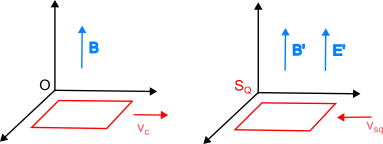
\includegraphics[width = 0.6 \textwidth]{images/relati.png}
\end{center}

Nella prima immagine partendo da sinistra abbiamo che 
\begin{equation}
	\bold{F_B} = q\bold{v_c} \times B \neq 0  
\end{equation}
mentre il campo elettrico \`e $E = 0 $. Da questo risultato possiamo dedurre che la corrente indotta che si osserva all'interno della spira deve essere conseguenza di una forza di natura magnetica. 

Se consideriamo la seconda immagine in cui $S_Q$ \`e  il sistema fissato, osserveremo il sistema O muoversi con velocit\`a $\bold{v_c}$ in senso opposto. Rispetto al sistema  $S_Q$ le cariche sono stazionare 
di conseguenza $F_{B'} = 0$ e quindi la corrente che si osserva all' interno della spira non pu\`o essere conseguenza di un effetto magnetico. Inoltre \`e presente un campo eletrico $E'$.

Nel seguente paragrafo delineiamo i principi che legano il campo magnetico variabile alle forze che permettono di osservare della corrente all'interno di un conduttore.
\section{Legge di Faraday}

Una delle equazioni di Maxwell mette in relazione campi magnetici ed elettrici 
\begin{equation}
	\nabla \times \bold{E} + \frac{\partial \bold{B}}{\partial t} = 0
\end{equation}
Tale equazione ci dice che che se il campo magnetico \`e variabile nel tempo, allora crea un campo elettrico. La creazione di un campo elettrico fa s\`i che le cariche vengano accelerate, ovvero creino una corrente all'interno di un filo. Il processo di creazione di una corrente mediante un campo magnetico variabile prende il nome di \textit{induzione}.

\begin{wrapfigure}{r}{0.4\textwidth} % 'r' for right, 'l' for left
    \centering
    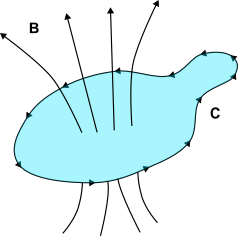
\includegraphics[width=0.32\textwidth]{images/faraday_law}
\end{wrapfigure}
Consideriamo un filo come un conduttore, avvolto attorno ad una curva stazionaria C. Un filo chiuso prende il nome di circuito. Se integriamo l'equazione (5.1) rispetto alla superficie S racchiusa dal circuito chiuso C, abbiamo che
\begin{equation*}
	\int_{S}(\nabla \times \bold{E}) \cdot d \bold{S} = - \int_{S} \frac{\partial \bold{B}}{\partial t} \cdot d\bold{S}
\end{equation*}
utilizzando il teorema di Stokes possiamo riscrivere l'equazione come
\begin{equation*}
	\oint_{C} \bold{E} \cdot d\bold{r} = - \int_{S} \frac{\partial \bold{B}}{\partial t} \cdot d \bold{S} = - \frac{d}{dt} \int_{S} \bold{B} \cdot d \bold{S}
\end{equation*}
Per ottenere l'ultima relazione abbiamo assunto che n\`e C e n\`e S possano cambiare nel tempo. L'integrale di linea attorno a C del campo elettrico prende il nome di \textit{forza elettromotrice}, $\mathcal{E}$, che di solito viene abbreviata con $fem$.
\begin{equation*}
	\mathcal{E} = \oint_{C} \bold{E} \cdot d \bold{r}
\end{equation*}
La forza elettromotrice non \`e realmente una forza come possiamo vedere dalla sua espressione, in realt\`a \`e la componente tangenziale della forza per unit\`a di carica, integrata lungo un filo. Un altro modo di vederla \`e dato dal lavoro necessario a spostare una carica unitaria lungo la curva C. Se la $fem$ \`e non nulla allora \`e presente della carica accelerata all'interno del filo che genera quindi una corrente.

L'integrale del campo magnetico passante attraverso la superficie S prende il nome di flusso magnetico $\Phi$ attraverso la superficie S,
\begin{equation*}
	\Phi = \int_{S} \bold{B} \cdot d\bold{S}
\end{equation*} 
Di conseguenza possiamo riscrivere l'equazione di Maxwell (5.1) come 
\begin{equation}
	\mathcal{E} = - \frac{d\Phi}{dt}
\end{equation}
In questa forma l'equazione prende il nome di \textit{legge di Faraday}. 
\newline

\noindent La legge di Faraday ci dice che se cambiamo il flusso del campo magnetico attraverso una superficie S delimitata da un circuito, allora osserveremo un flusso di corrente all'interno del filo. Esistono diversi modi per modificare il campo magnetico, per esempio spostando una barra magnetica in vicinanza ad un circuito, passandola attraverso la superficie S delimitata dal filo conduttore. Un altro modo \`e dato muovendo un secondo filo $C''$ attraverso da una corrente, oppure tenendolo fisso e variando l'intensit\`a di corrente al suo interno accendendolo e spegnendolo. Tutti questi metodi inducono una corrente in C.
\newline

Esiste anche un secondo effetto, dovuto al fatto che dato un campo magnetico variabile e avendo una corrente indotta all'interno del circuito C, avremo che a sua volta la carica in moto genera un suo campo magnetico. Il campo magnetico indotto \`e orientato sempre in opposizione al cambiamento. Questo fenomeno prende il nome di \textit{legge di Lenz} e giustifica il segno negativo nella legge di Faraday (5.2). 

\subsection{Legge di Lenz}

 Il segno meno che compare nell'espressione (5.3) \`e molto importante in quanto mette in evidenza il fatto che l'effetto della $fem$ indotta \`e sempre tale da opporsi alla causa che ha generato il fenomeno.
\begin{center}
	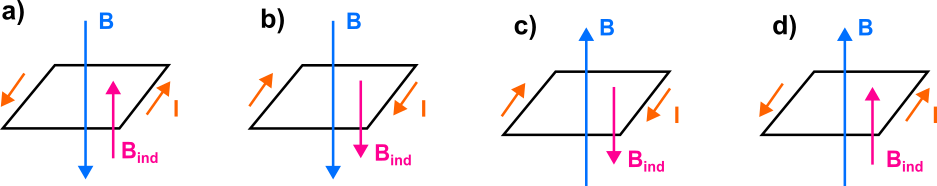
\includegraphics[width = 15cm]{images/lenz_law1}
\end{center}
Possiamo riassumere i casi possibili nelle quattro configurazioni in figura:
\begin{enumerate}
	\item a)il flusso del campo magnetico $d\phi/dt >0 $, di conseguenza $\mathcal{E} <0$ e viene generata una corrente in senso $antiorario$ che produce un campo magnetico $\bold{B} _{ind}$ indotto. In questo modo si ottiene un autoflusso che si oppone all'aumento di $\phi(\bold{B}_{ind})$, cos\`i che il flusso complessivo attraverso il circuito cresce  pi\`u lentamente.
	\item b) il flusso del campo magnetico \`e ($d\phi/ dt < 0 $) la fem indotta \`e $\mathcal{E} > 0$. La corrente nel circuito scorre in senso $orario$, si genera un campo magnetico indotto concorde con il campo esterno. L'autoflusso si oppone alla diminuzione e in questo modo il flusso complessivo decresce pi\`u lentamente.
	\item c) e d) sono l'equivalente di a) e b), ma con direzione del campo esterno opposta. 
\end{enumerate}
\subsection{Esempio: Batteria (Corrente Stazionaria)}

Quando osserviamo della corrente all'interno di un circuito ci sono solo  due forze responsabili del trasporto delle cariche: la sorgente, $\bold{F_s}$, che solitamente  \`e confinata in una porzione del circuito (come una batteria) e una forza di natura elettrostatica, che serve a trasportare l'effetto della sorgente sul  resto del circuito:
\begin{equation}
	\bold{F} = \bold{F_s}  + \bold{E}
\end{equation}
Nel caso di una batteria $\bold{F_s}$ \`e data dal potenziale chimico al suo interno. Il lavoro compiuto complessivamente sul circuito \`e dato come sempre dall'integrale di linea della forza agente su di esso quindi 
\begin{equation*}
	\mathcal{E} \equiv \int_{C} \bold{F} \cdot \bold{ds} = \int_C  \bold{F_s}  \cdot \bold{ds}
\end{equation*}

e quindi come definito il precedente all'interno del circuito  abbiamo una forza elettromotrice responsabile de flusso delle cariche al suo interno.  

Se consideriamo un modello semplificato della batteria, in cui ne trascuriamo la resistenza,  abbiamo che la forza sulle cariche \`e  $E = -\bold{F_s} $, dunque la \textit{fem} possiamo vederla legata alla tensione ai campi della batteria.
\begin{equation*}
	\mathcal{E} = \int_{C} \bold{F_s} \cdot \bold{ds} = - \int_{a}^b \bold{E} \cdot \bold{dl} = V
\end{equation*}

Lo scopo di una batteria \`e  quello di mantenere un differenza di potenziale all'interno di un circuito pari alla forza elettromotrice. Notare che all'interno di una batteria $\bold{F_s}$ la corrente ha flusso in direzione opposta al campo elettrico $\bold{E}$.


\subsection{Generatori Elettrici}

Ipotizziamo di avere un sistema in cui abbiamo una sorgente (generatore) che genera un campo magnetico $\bold{B}$ stazionario, ma non uniforme nello spazio. Nel sistema \`e presente una spira rettangolare in moto con velocit\`a $\bold{v}$ costante.

\begin{center}
	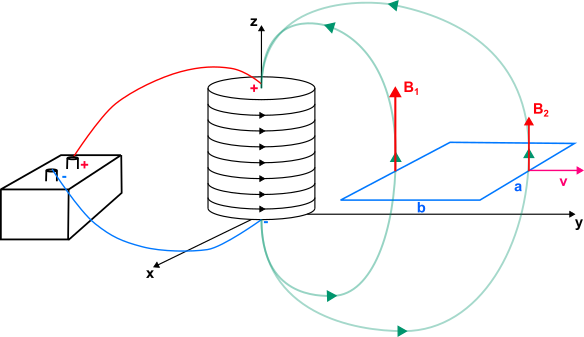
\includegraphics[width = 0.6 \textwidth]{images/generator.png}
\end{center}

Siccome il campo magnetico $\bold{B} = \bold{B}(\bold{r})$ dipende dalla poszione la forza a cui sono soggette le cariche nella spira dipende dalla distanza dalla sorgente. Calcolando la forza di Lorenetz  per unit\`a di carica  $\bold{F_B} = \bold{v} \times \bold{B}$, ad un istante di tempo t:
\begin{equation*}
	\oint \bold{F_B} \cdot \bold{ds} = v(B_1 - B_2)a \neq 0 
\end{equation*}
dove $a$ \`e la lunghezza di un tratto della spira.  Lungo $b$ la forza $\bold{F_B}$ \`e ortogonale al tratto di spira (vedere figura) di conseguenza non contribusce all'intergrale, e quindi si un constributo solo lungo $a$ dove $\bold{F_B}$ \`e parallelo alla direzione.

La forza complessiva che agisce su una carica  del circuito \`e data da 
\begin{equation*}
	\bold{F} = q \bold{v} \times \bold{B} + q\bold{E}
\end{equation*}

di conseguenza il lavoro compiuto dal generatore \`e dato da 
\begin{equation*}
	\mathcal{E} = \oint \bold{f} \cdot \bold{ds} = \oint (\bold{v} \times \bold{B} + \bold{E}) \cdot \bold{ds} = \oint (\bold{v} \times \bold{B}) \cdot \bold{ds}
\end{equation*}
dove si \`e trascurato il contributo del campo elettrico $\bold{E}$ essendo conservativo. Il lavoro compiuto dal generatore \`e  proprio la forza elettromotrice che permette lo spostamento delle carriche e coincide con la forza di Lorentz per unit\`a di carica.

\subsection{Moto di un filo in un campo magnetico stazionario}

\begin{wrapfigure}{r}{0.4\textwidth} % 'r' for right, 'l' for left, width of the figure
    \centering
    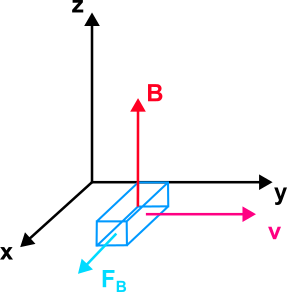
\includegraphics[width=0.35\textwidth]{images/barra.png} % Replace with your image
\end{wrapfigure}
Come abbiamo visto un modo per indurre una corrente all'interno un conduttore \`e  quello di mantere la sorgente fissata e il conduttore in moto. Se prendiamo come conduttore una barra di lunghezza $a$ (o segmento di circuito), le cariche libere si muovono sotto l'azione di $\bold{F_B} = q \bold{v} \times \bold{B}$.
sulle cariche si raggiunge uno stato di equilibrio statico quondo il campo $\bold{E}$ interno al conduttore, generato dalla distribuzione di carica, ottenuta doopo il riarrangiamento indotto da $\bold{F_B}$, bilancia la forza di Lorentz.
\begin{equation*}
	\bold{F_B} + \bold{F_E} = 0 \iff \bold{E} = - (\bold{v} \times \bold{B})
\end{equation*}  
Ai capi della barra compare una differenza di potenziale

\begin{equation*}
	\Delta V  = - \int_{0}^{a} \bold{E} \cdot \bold{ds} = \int_0^{a}(\bold{v} \times \bold{B}) \cdot \bold{ds}
\end{equation*}

Se il circuito \`e chiuso, se $\bold{B}$ non \`e uniforme, abbiamo che $\Delta V_1 \neq \Delta V_2$ nei due segmenti distanti tra loro, di conseguenza compare una $fem$, dovuta alla forza di Lorentz.

\subsection{Lavoro della forza esterna }

Prendiamo un sistema in cui \`e presente un campo magnetico $\bold{B}(\bold{r})$ non uniforme e al suo interno \`e  immersa una spira rettangolare di lato minore $a$ (il lato maggiore non ci interessa per la dinamica del problema). Ipotizziamo che la spira sia tirata da una forza esterna $\bold{F_ext}$ concorde con gli assi del 
sistema di riferimento. 
\begin{center}
	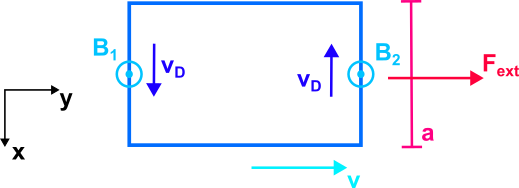
\includegraphics[width = 0.6 \textwidth]{images/lavoro.png}
\end{center}
All'interno della spira \`e presenta una corrente di cariche che si spostano con velocit\`a $\bold{v}_D$ che \`e la velocit\`a di deriva e una componente di velocit\`a $\bold{v}$ data dalla forza esterna agente. La velocit\`a di una singola carica \`e quindi data da
\begin{equation*}
	\bold{v}_q =  v_D \bold{\hat{\mu}_x}  + v \bold{\hat{\mu}_y}
\end{equation*}

La forza sulle cariche presenti nei due segmenti verticali alla direzione di spostamento che contribuiscono al lavoro \`e data da 
\begin{equation*}
	\bold{F_1} = q \bold{v} \times \bold{B_1} = \underbrace{-q \bold{v_D}B_1 \bold{\hat{\mu}_y}}_{\text{opposta a } \bold{F_{ext}} } + qvB_1 \hat{\mu}_x
\end{equation*}
il secondo addendo determina il moto delle cariche nel filo. Affinch\`e la spira si sposti con moto rettilineo uniforme lungo $\hat{\mu}_y$ abbiamo bisogno che la risultate delle forze sulla spira (e quindi sulle cariche) sia $\bold{R} = 0$ il che equivale a 
\begin{equation*}
	\bold{F_{ext}} = -q v_D(B_1-B_2)\hat{\mu}_y
\end{equation*}
per uno spostamento $\Delta y$ il lavoro compiuto dalla forza esterna \`e dato da 
\begin{equation*}
	W_{ext} =qv_D(B_1-B_2)\Delta y
\end{equation*}
Le cariche in un tempo $\Delta t$ si muovono lungo gli assi percorrendo le distante 
\begin{equation*}
a = v_D \Delta t \quad \text{e} \quad \Delta y = v \Delta t
\end{equation*} 
sostituendo per i tempi otteniamo la relazione $v_D \Delta y = a v$ e quindi possiamo scrivere la forza esterna come 
\begin{equation*}
	W_{ext} = q v(B_1-B_2)a
\end{equation*}
In questo modo si dimostra che la forza responsabile della corrente nel circuito \`e la forza esterna che alimenta la forza elettromotrice.

\subsection{Caso Generale }
\begin{wrapfigure}{r}{0.4\textwidth} % 'r' for right, 'l' for left
    \centering
    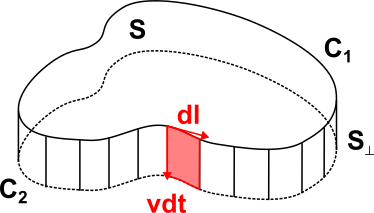
\includegraphics[width=0.38\textwidth]{images/flux_theorem.png} % Replace with your image
\end{wrapfigure}

Esiste un modo semplice per dimostrare la relazione tra forza elettromotrice e variazione di flusso di un campo magnetico che cambia nel tempo. Ipotizziamo di avere un generico circuito $C(t)$ che pu\`o essere mosso rigidamente e attraversato da un campo magnetico $\bold{B}$. Al tempo $t + \delta t$ il circuito \`e stato traslato in una nuova posizione, questo porta ad avere un cambio del flusso del campo $\bold{B}$ di conseguenza possiamo scrivere 
\begin{equation*}
	d \phi = \phi(t + \delta t) - \phi(t) = \int_{S(t+ \delta t)} \bold{B}(t+\delta t) \cdot d\bold{S} - \int_{S(t)} \bold{B}(t) \cdot d\bold{S}
\end{equation*}
notare che siccome il movimento del circuito \`e rigido la superficie rimane la medesima durante lo spostamento.

Sviluppando con Taylor il campo magnetico abbiamo che 
\begin{equation}
	d \phi = \int_{S(t)} \frac{\partial \bold{B}}{\partial t}dt \cdot d \bold{S} + \left[\int_{S(t+\delta t)} - \int _{S(t)}\right]\bold{B}(t) \cdot d\bold{S} + \mathcal{O}(\delta t^2)
\end{equation}

Il termine $\int_{S(t+ \delta t)} - \int_{S(t)}$ rappresenta una superficie chiusa  formata dal volume compreso nella regione di traslazione rigida del cammino, il contorno di tale regione lo definiamo $S_C$. Dato che il campo magnetico \`e  irrotazionale $\nabla \cdot \bold{B} = 0$ l'integrale di $\bold{B}(t)$ su una qualsiasi superficie chiusa risulta essere nullo. Per questo motivo complessivamente dobbiamo avere 
\begin{equation*}
	\left[\int_{S(t + \delta t)} - \int_{S(t)}\right] \bold{B}(t) \cdot d\bold{S} + \int_{S_C} \bold{B}(t) \cdot d \bold{S} = 0  
\end{equation*}
e quindi 
\begin{equation*}
\left[\int_{S(t + \delta t)} - \int_{S(t)}\right] \bold{B}(t) \cdot d\bold{S} = -\int_{S_C} \bold{B}(t) \cdot d \bold{S}  
\end{equation*}
Un elemento di superficie di $S_C$ \`e dato da 
\begin{equation*}
	d\bold{S} = (d\bold{r} \times \bold{v}) \delta t
\end{equation*} 
dove d$\bold{r}$ \`e un tratto del circuito $C(t)$ e $\bold{v}dt$ il tratto di cui si \`e stato traslato in un tempo $\delta t$.

Di conseguenza l'equazione (5.5) pu\`o essere riscritta nel seguente modo
\begin{equation}
	\frac{d\phi }{dt } = \int_{S(t)}\frac{\partial \bold{B}}{\partial t} \cdot d\bold{S} - \int_{C(t)}(\bold{v} \times \bold{B})\cdot d\bold{r}
\end{equation}
dove abbiamo usato la propriet\`a per i prodotti misti per riscrivere $(d\bold{r} \times \bold{v} ) \cdot \bold{B} = d\bold{r} \cdot (\bold{v} \times \bold{B})$. Dall'equazione di Maxwell sappiamo che 
\begin{equation*}
	\nabla \times \bold{E} = \frac{\partial \bold{B}}{\partial t} 
\end{equation*}
abbiamo che (5.6) diventa 
\begin{equation*}
	\frac{d\phi}{dt} = - \int_{C} (\bold{E}+\bold{v} \times \bold{B}) \cdot d\bold{r} 
\end{equation*}
Il termine di destra include la forza tangenziale al filo data sia dal campo elettrico che dallo spostamento del filo in presenza di un campo magnetico. Tale relazione che tiene conto di entrambi i contributi definisce la forza elettromotrice 
\begin{equation}
	\mathcal{E} = \int_{C}(\bold{E} + \bold{v} \times \bold{B}) \cdot d \bold{r}
\end{equation}
e quindi ritroviamo la legge del flusso definita ad inizio capitolo $\mathcal{E} = - d\phi /dt$.

La forza elettromotrice \`e omogenea alla differenza di potenziale, in elettrodinamica (o nei circuiti con correnti non stazionarie) questa viene definita differenza di tensione $\Delta V$ in quanto il campo elettrico $\bold{E}$ non \`e conservativo e non ammette potenziale. Come conseguenza la tensione elettrica dipende dal percorso.
\newpage

\subsection{Esempio: Generatore di Corrente Alternata }

\begin{wrapfigure}{l}{0.4\textwidth} % 'r' for right, 'l' for left
    \centering
    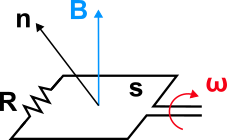
\includegraphics[width=0.30\textwidth]{images/alt_gen.png} % Replace with your image
\end{wrapfigure}

Dato un circuito chiuso C chiuso in cui \`e presente una resistenza R, questo viene messo in rotazione rispetto all'asse orizzontale passante per esso con velocit\`a angolare costante $\omega$, inoltre inizialmente il cammino forma un angolo $\theta_0$ rispetto al versore $\hat{\mu}_z$. All'interno del sistema \`e presente un campo magnetico $\bold{B} = B \hat{\mu}_z$ stazionario in cui la spira \`e immersa. Determinare la corrente che scorre all'interno del circuito.

\begin{proof}
	\begin{equation*}
		\phi_{S} (\bold{B}) = \bold{B} \cdot S\hat{\bold{n}} = BS\cos(\omega t + \theta_0)
	\end{equation*}
Usando la legge di Faraday
\begin{equation*}
	\mathcal{E} = - \frac{d \phi}{dt} = \omega BS\sin(\omega t+\theta_0) 
\end{equation*}
Dato che la forza elettromotrice coincide con la differenza di tensione alle estremit\`a del circuito e per ipotesi il materiale di cui \`e composto \`e ohmnico possiamo usare la legge $V = RI$ e quindi 
\begin{equation*}
	I(t) = \frac{\mathcal{E}}{R}
\end{equation*}
\end{proof}

\subsection{Esempio: Dinamo di Faraday}

\begin{wrapfigure}{r}{0.4\textwidth} % 'r' for right, 'l' for left
    \centering
    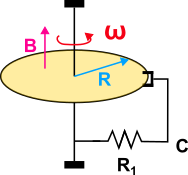
\includegraphics[width=0.30\textwidth]{images/faraday_dinamo.png} % Replace with your image
\end{wrapfigure}
Un disco di metallo di raggio R ruota con velocit\`a angolare $\omega$ rispetto all'asse verticale passante per il centro. Il mezzo conduttore si trova immerso in un campo magnetico $\bold{B}$ con direzione e orientamento parallelo all'asse di rotazione del disco. Si costruisce un circuito collegando ad un capo dell'asse una resistenza e al disco un contatto che ne permetta la rotazione. Determinare la corrente nel conduttore.

\begin{proof}
	In questo caso non \`e possibile utilizzare la definizione della forza elettromotrice rispetto al flusso del campo magnetico, siccome questo risulta essere nullo attraverso la superficie del conduttore, inoltre non \`e possibile dedurre quale sia il percorso della corrente al suo interno. In questi casi \`e meglio utilizzare la definizione di forza elettromotrice come lavoro della forza di spostamento delle cariche lungo un cammino.
	\begin{equation*}
		\mathcal{E} = \oint \bold{F_s} \cdot d \bold{l} 
	\end{equation*}
Dato che le cariche si muovono in modo uniforme, abbiamo che la risultante delle forze su di esse \`e nulla $\bold{R} = 0$ e quindi $\bold{F_s} = \bold{F_{B}}$ dove $\bold{F}_{B}$ \`e la forza di Lorentz. La velocit\`a delle cariche \`e data da $\bold{v}_q = \omega t \hat{u}_\theta$ e quindi 
\begin{equation*}
	\bold{f}_B = \bold{v}_q \times \bold{B} = \omega r B \hat{\mu}_r
\end{equation*}
e quindi 
\begin{equation*}
	\mathcal{E} = \oint \bold{f_{B}} \cdot d \bold{l} = \int_{0}^{R} \omega rBdr = \frac{1}{2}\omega BR^2
\end{equation*}

\end{proof} 

\subsection{Sorgenti magnetiche  in moto (Secondo Esperimento di Faraday)}

Consideriamo un sistema di riferimento $O$ solidale con la sorgente di campo magnetico e un sistema di riferimento $O'$ solidale con una spira chiusa che si sposta lungo una direzione con veloict\`a $\bold{v}$. Per la relativit\`a  classica il sistema O risulta essere in moto relativo rispetto alla spira, e in entrambi i sistemi si deve osservare lo stesso fenomeno, ovvero della corrente indotta all'interno del circuito dovuta alla forza elettromotrice $\mathcal{E}$ o $\mathcal{E}'$ a seconda del riferimento.

L'interpretazione della natura della forza elettromotrice per\`o  risulta essere differente, infatti in $O'$ non ci sono forze magnetiche poich\`e rispetto ad essa le cariche risultano essere ferme. Dalla definizione di forza elettromotrice data da (5.7) sappiamo che in generale 
\begin{equation*}
	\mathcal{E} = \oint \bold{f_s} \cdot d\bold{l} = \oint (\bold{E} + \bold{v} \times \bold{B}) \cdot d \bold{l}
\end{equation*} 
se calcoliamo la forma elettromotrice rispetto al riferimento della spira $O'$ 
\begin{equation*}
	\mathcal{E}' = \oint \bold{E}' \cdot d\bold{r}
\end{equation*}   
quindi in virt\`u di quanto osservato sperimentalmente deve esistere un campo elettrico $\bold{E}'$ rispetto a cui la circuitazione non \`e nulla (si ha un caso non elettrostatico).

Per semplicit\`a  consideriamo solo lo spostamento di un segmento del circuito (sbarra conduttrice).

\begin{center}
	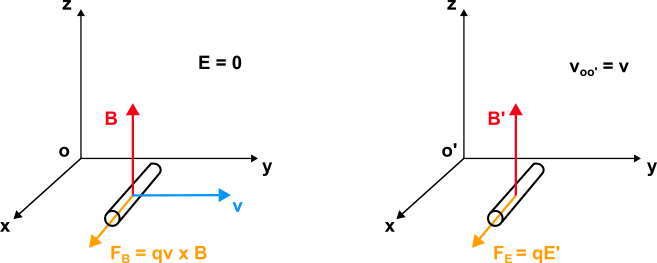
\includegraphics[width = 15cm]{images/rel_bar.png}
\end{center}
Nel riferimento $O'$ solidale con la sbarra in moto relativo a O, con velocit\`a $v_{OO'} = v$, per determinare il campo elettrico $\bold{E'}$ utilizziamo le seguente leggi di trasformazione di campo
\begin{align}
\left \{ \begin{array}{l}
	\bold{E'}_{\parallel} = \bold{E}_{\parallel} \\ \rule{0pt}{20pt}
	\bold{B'}_{\parallel} = \bold{B}_{\parallel}
\end{array}	\right.
\quad \quad
\left \{ \begin{array}{l}
	\bold{E'}_{\perp} = \gamma (\bold{E}_{\perp} + \bold{v} \times \bold{B}_{\perp}) \\ \rule{0pt}{20pt}
	\bold{B'}_{\perp} = \gamma \left(\bold{B}_{\perp} - \frac{\bold{v} \times \bold{E}_{\perp}}{c^2} \right)
\end{array}	\right. 
\end{align}
Dato che in O $\bold{E} = 0$ e $\bold{B}_{\parallel} = 0$, in $O'$ si ha che :
\begin{align}
	\left \{ \begin{array}{l}
		\bold{B}' = \gamma \bold{B}_{\perp} \\ \rule {0pt}{20pt}
		\bold{E}' = \gamma (\bold{v} \times \bold{B}_{\perp}) = \bold{v} \times \bold{B}' 
	\end{array}\right.
\end{align}
In $O'$ le cariche libere nel conduttore si dispongono in modo da annullare il campo elettrico all'interno del conduttore 
\begin{equation*}
	\bold{E}'_{cond} = \bold{E}' + \bold{E}_{ind} = 0 \Rightarrow  \bold{E}_{ind} = -\bold{E}' =-\bold{v} \times \bold{B}'
\end{equation*}
in questo modo si ha la condizione elettrostatica in cui $\bold{v}_q = 0$.

Nel sistema di riferimento O si giunge a un risultato analogo dove affinch\`e le cariche si muovano di moto uniforme 
\begin{equation*}
	\bold{f} = \bold{E} + \bold{v} \times \bold{B} = 0 \Rightarrow \bold{E} = -\bold{v} \times \bold{B}
\end{equation*}
internamente al conduttore.
\begin{center}
	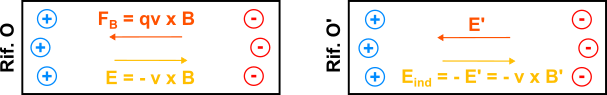
\includegraphics[width = 15cm]{images/riferiment.png}
\end{center}
I due osservatori interpretano diversamente i fenomeni e vedono campi $\bold{E}$ e $\bold{B}$ differenti, ma osservano il medesimo risultato sperimentale, questo \`e dovuto al fatto che la distribuzione di carica \`e la medesima.

\subsubsection{Calcolo della Forza Elettromotrice nel sistema O'}

\begin{wrapfigure}{r}{0.4\textwidth}  % 'r' for right, 'l' for left
    \centering
    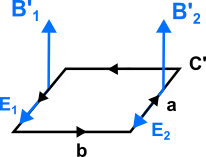
\includegraphics[width=0.38\textwidth]{images/move_charge} % Replace with your image file
\end{wrapfigure}

Ora che abbiamo determinato l'espressione del campo elettrico nel sistema di riferimento $O'$ possiamo procedere a calcolarne esplicitamente la forza elettromotrice indotta sulla spira quadrata considerata inizialmente.

Ipotizziamo che il campo magnetico in cui \`e immersa la spira sia non uniforme, di conseguenza il campo elettrico indotto $\bold{E}'$ avr\`a  verso e intensit\`a  differente rispetto al tratto della spira considerato. Lungo il lato maggiore del circuito il campo \`e ortogonale allo spostamento di conseguenza non contribuisce all'integrale di linea con cui calcoliamo la forza elettromotrice 
\begin{equation*}
	\mathcal{E}' = \oint \bold{E}' \cdot d\bold{l} = E_1'a  + E_2'(-a) = v(B_1' - B_2')a
\end{equation*}
Il calcolo del flusso, geometrico, \`e identico nei due sistemi di riferimento infatti 
\begin{equation*}
	\frac{d \phi '}{dt'} = - va(B_1'-B_2') = - \mathcal{E}' \Rightarrow \mathcal{E}' = - \frac{d\phi'}{dt'}
\end{equation*} 

La relazione del flusso del campo magnetico con la forza elettromotrice \`e  invariante in forma, nonostante i due osservatori ne abbiano un'interpretazione fisica differente.
\begin{enumerate}
	\item Nel sistema di riferimento $O$ \`e la forza magnetica e quindi $\mathcal{E}= \oint \bold{f_B} \cdot d \bold{l} $ 
	\item Nel sistema di riferimento $O'$ \`e il campo elettrico indotto $\mathcal{E}' = \oint \bold{f_E'} \cdot d \bold{l}$
\end{enumerate}
\begin{center}
\fbox{\parbox{12cm}{
\textit{Un campo magnetico variabile sull'area del circuito induce un campo elettrico non conservativo responsabile della forza elettromotrice.}}}
 \end{center}
 Faraday ottiene questa relazione per via empirica. 
\begin{remark}

 Nell'esempio considerato il campo $\bold{B}$ \`e stazionario e in moto relativo, ma \`e variabile nel riferimento del laboratorio (solidale con la spira), eccetto nel caso in cui $\bold{B}$ \`e uniforme 
\end{remark}

\subsection{Campo Magnetico Variabile (Terzo Esperimento di Faraday)}

Abbiamo visto come per un circuito in moto rispetto alle sorgenti e viceversa la forza elettromotrice ha origini differenti rispetto all'osservatore, ma la legge di Faraday rimane comunque un invariante relativistico in forma. Nel paragrafo precedente per l'osservatore del laboratorio solidale con la spira per giustificare la fisica del fenomeno abbiamo introdotto un campo elettrico indotto, la giustificazione della sua introduzione \`e chiara solo in relativit\`a speciale.

Faraday compie un terzo esperimento in cui osserva una corrente all'interno di un conduttore, ovvero mantiene sorgenti e circuito statici e varia il campo magnetico $\bold{B}$. Sperimentalmente osserva che a medesime variazioni di $\bold{B}$ sulla spira indotte:
\begin{enumerate}
	\item spostando le sorgenti 
	\item modificando l'intensit\`a del campo.
\end{enumerate} 
corrispondono medesime correnti indotte. Questo ci permette di dedurre che 
\begin{center}
\fbox{\parbox{12cm}{
\textit{La forza elettromotrice indotta localmente dipende solo dalle variazioni locali del flusso e non dalla natura delle sorgenti.}}}
\end{center}
Per quanto ragionevole questo \`e un risultato sperimentale che non pu\`o essere dedotto per via analitica, a differenza del secondo esperimento la cui natura del campo elettrico indotto pu\`o essere giustificato dalla relativit\`a speciale.

\subsection{Legge di induzione di Faraday per Campi Magnetici Stazionari}

Per ogni linea chiusa C, stazionaria nelle coordinate,  se $\bold{B}$ \`e il campo misurato al tempo t, vale la relazione 
\begin{equation*}
	\mathcal{E} = - \frac{d\phi}{dt}
\end{equation*}
dove 
\begin{align}
	\left \{ \begin{array}{l}
		\phi(\bold{B}) = \int_{S} \bold{B} \cdot d\bold{A} \\ \rule{0pt}{20pt}
		\mathcal{E} = \oint_C \bold{E} \cdot d \bold{l}
	\end{array}\right .
\end{align} 
Lo specificare la stazionariet\`a nelle coordinate significa che la Legge di Faraday descrive a rigore soli il secondo e terzo esperimento di Faraday. Nel caso di un circuito variabile immerso in un campo $\bold{B}$ stazionario la fem \`e dovuta a $\bold{f_B}$, e non vale l'espressione della forza elettromotrice in (5.10). In questo caso si ricorre alla regola universale del flusso in (5.7).

\subsection{Esempio: Variazione del Campo Mangnetico}

\begin{wrapfigure}{l}{0.4\textwidth}  % 'r' for right, 'l' for left
    \centering
    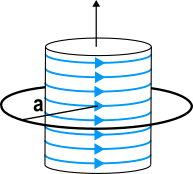
\includegraphics[width=0.32\textwidth]{images/solenoid_spire} % Replace with your image file
\end{wrapfigure}

Consideriamo un sistema costituito da una solenoide di raggio b, densit\`a di spire $n$ e attraversato da una corrente $I(t) = I_0 \cos(\omega t)$ intorno al quale \`e posta una spira di raggio $a$ e resistenza $R$. Determinare la forza elettromotrice indotta nel circuito.

\begin{proof}
	Il campo magnetico generato dal solenoide attraversato dalla corrente \`e dato da 
	\begin{equation*}
		\bold{B}(t) = \mu_0 nI(t) \hat{\bold{u}}_z \quad r<b
	\end{equation*}
utilizzando la legge di Fataday che lega $fem$ e variazione del flusso del campo magnetico abbiamo che 
\begin{equation*}
	\mathcal{E} = - \frac{d}{dt}(B(t) \pi b^2) = -\pi b^2 \frac{dB}{dt} = \pi b^2 \omega \mu_0 n \omega I_0 \sin(\omega t)
\end{equation*}
\end{proof}

\subsection{Esempio: Circuito e Campo magnetico variabili}

Consideriamo un sistema in cui sia il campo magnetico che il circuito cambiano nel tempo avremo che la variazione di flusso \`e data da
\begin{align*}
	d \phi & = \int_{S(t + dt)} \bold{B}(t + dt) \cdot d \bold{A} - \int_{S(t)} \bold{B}(t) \cdot d\bold{A} = \\ \rule{0pt}{30pt}
	& =\int_{S(t+dt)}\left[ \bold{B}(t) + \frac{\partial \bold{B}}{\partial t}\right] \cdot d \bold{A} - \int_{S(t)} \bold{B}(t) \cdot d\bold{A} = \\ \rule{0pt}{30pt}
	& = \left[\int_{S(t+dt)} - \int_{S(t)}\right] \bold{B}(t) \cdot d\bold{A} +\int_{S(t)} \frac{\partial \bold{B}}{\partial t} dt \cdot d\bold{A} = \\ \rule{0pt}{30pt}
	& \Rightarrow \frac{d \phi }{dt } = - \bold{B}(t) \frac{dS}{dt} - \int_{S} \frac{\partial \bold{B}}{\partial t} \cdot d \bold{A} 
\end{align*}
Il primo termine \`e legato alla forza elettromotrice data dalla forza magnetica mentre il secondo da quella data dal campo elettrico. 

Il campo elettrico della legge di Faraday per il secondo e terzo esperimento indotto da un campo magnetico $\bold{B}(t)$ variabile, esiste anche in assenza di un circuito materiale:
\begin{enumerate}
	\item La linea chiusa C formata da un circuito pu\`o essere immateriale;
	\item Se lungo C \`e disposto un conduttore o delle cariche libere, il campo $\bold{E}$ si manifesta con una corrente indotta.
\end{enumerate}

\subsection{Forma Locale della Legge di Faraday}
Ad inizio capitolo si \`e dimostrata la legge di Faraday assumendo gi\`a l'espressione in forma locale, ma come la si ottiene ?

Abbiamo visto come nel caso del secondo e terzo esperimento di Faraday possiamo condensare la relazione tra campo elettrico e campo magnetico variabile 
\begin{equation*}
	\oint_{C} \bold{E} \cdot d\bold{l} = - \frac{d}{dt} \int_{S} \bold{B} \cdot d\bold{A}
\end{equation*}
Per esprimere la relazione in forma locale, prendiamo una linea chiusa molto piccola e utilizziamo il teorema di Stokes 
\begin{equation*}
	\int_{S} (\nabla \times \bold{E}) \cdot d\bold{A} = - \frac{d}{dt} \int_{S} \bold{B} \cdot d\bold{A}
\end{equation*}
ottenendo la \textit{legge di Faraday in forma locale}. Dato che C \`e molto piccolo anche la superficie S sar\`a molto piccola e di conseguenza possiamo assumere che $\bold{B}$ e $\nabla \times \bold{E}$ siano costanti su di essa.
\begin{equation*}
	(\nabla \times \bold{E}) \cdot \bold{S} = - \frac{d}{dt}(\bold{B} \cdot \bold{S})
\end{equation*}
Dato che S \`e indipendente dal tempo vale l'identit\`a 
\begin{equation*}
	\nabla \times \bold{E} = - \frac{\partial \bold{B}}{\partial t}
\end{equation*}
che prende il nome di \textit{forma differenziale della legge di Faraday}.

La forma differenziale della legge di Faraday, include il limite stazionario e il caso del primo esperimento di Faraday. Se il campo magnetico $\bold{B}$ non dipende dal tempo, il campo elettrico \`e conservativo, ossia $\nabla \times \bold{E}$. Dunque la forma differenziale della legge di Faraday \`e universale.

\subsection{Campo Elettrico Indotto}

La legge di Faraday generalizza la  condizione dell'elettrostatica  $\nabla \times \bold{E} = 0$ definendo una relazione locale tra il campo magnetico $\bold{B}$ e il campo elettrico $\bold{E}$ a meno di un campo elettrostatico $\bold{E}_0$, infatti se consideriamo 
\begin{align*}
	\nabla \times \bold{E}_1 = - \frac{\partial \bold{B}}{\partial t} \quad \text{e} \quad \nabla \times \bold{E}_0 = 0
\end{align*}
allora possiamo definire un campo $\bold{E}_2$ tale che 
\begin{equation*}
	\nabla \times \bold{E}_2 = - \frac{\partial \bold{B}}{\partial t} \quad \text{dove} \quad \bold{E}_2 = \bold{E}_1 + \bold{E}_0
\end{equation*}
Il campo elettrico complessivo \`e definito dalle relazione in forma differenziale 
\begin{align*}
	\left \{ \begin{array}{l}
		\nabla \cdot \bold{E} = \frac{\rho}{\varepsilon_0} \quad \text{Legge di Gauss} \\ \rule{0pt}{30pt}
		\nabla \times \bold{E} = - \frac{\partial \bold{B}}{\partial t} \quad \text{Legge di Faraday}
	\end{array}\right.
\end{align*}

Se il campo \`e puramente indotto ($\rho = 0$), le equazioni che definiscono il campo sono matematicamente identiche alle equazioni della magnetostatica.
\begin{align*}
	\left \{ \begin{array}{l}
	\nabla \cdot \bold{E} = 0 \\ \rule{0pt}{20pt} 
	\nabla \times \bold{E} = - \frac{\partial \bold{B}}{\partial t}		
	\end{array}\right.
	\quad \quad  
	\left \{ \begin{array}{l}
	\nabla \cdot \bold{B} = 0 \\ \rule{0pt}{20pt} 
	\nabla \times \bold{B} = \mu_0 \bold{J}		
	\end{array}\right.
\end{align*}
e dunque si hanno le stesse soluzioni 
\begin{equation*}
	\bold{E} = - \frac{1}{4 \pi } \frac{\partial}{\partial t} \int_{V} \frac{\bold{B} \times \bold{\hat{u}_r}}{|\bold{r} - \bold{r}'|}d \nu \quad \quad \text{Biot-Savart}
\end{equation*}

\subsubsection{Simmetrie e Legge di Faraday}
Se i campi presentano delle simmetrie risulta comodo utilizzare la forma integrale della legge di Faraday e ricorrere alle stesse strategie sviluppate con la legge di Amp\'ere :
\begin{equation*}
	\oint_{C} \bold{E} \cdot d\bold{l} = \bold{E} \cdot \oint_{C}d\bold{l} = - \frac{d \phi}{dt}
\end{equation*}
per un campo $\bold{E}$ costante sulla linea C ad un tempo fissato.
\subsection{Esempio 1 }
\begin{wrapfigure}{l}{0.4\textwidth}  % 'r' for right, 'l' for left
    \centering
    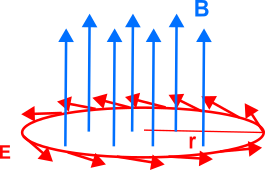
\includegraphics[width=0.32\textwidth]{images/change_field} % Replace with your image file
\end{wrapfigure}

Consideriamo un campo magnetico $\bold{B}(t) = B_0(t) \hat{\bold{u}}_z$ variabile nel tempo, uniforme nello spazio e a simmetria cilindrica. Questo induce un campo elettrico $\bold{E}= E(r) \hat{\bold{u}}_{\theta}$ nel piano,  ortogonale a $\bold{\hat{u}}_z$, e uniforme lungo il circuito. Dalla forma integrale della legge di Faraday
\begin{equation*}
	\mathcal{E} = \oint_{C} \bold{E} \cdot d \bold{l} = E_{\theta}(r,t) 2 \pi r = - \frac{\partial B}{\partial t} \pi r^2 
\end{equation*}
il campo elettrico  \`e dunque dato da 
\begin{equation*}
	E(r,t) = - \frac{1}{2} \frac{\partial \bold{B}}{\partial t} r \hat{\bold{u}}_{\theta} 
\end{equation*}
crescente linearmente con r.

\begin{remark}
\
\begin{enumerate}
	\item Se lungo r c'\`e una spira conduttrice 	 allora la corrente indotte \`e data da $\bold{J} = \sigma \bold{E}$.
	\item Il campo $\bold{E}(t)$ trovato \`e solo la componente associata a $\bold{B}$ variabile, al netto di eventuali campi elettrostatici sovrapposti.
\end{enumerate}
\end{remark}

\subsection{Esempio 2}

\begin{wrapfigure}{r}{0.4\textwidth}  % 'r' for right, 'l' for left
    \centering
    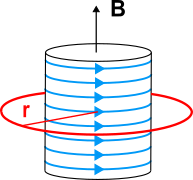
\includegraphics[width=0.32\textwidth]{images/solenoid1} % Replace with your image file
\end{wrapfigure}
Consideriamo il campo magnetico prodotto da un solenoide di raggio b attraversato da della corrente d'intensit\`a $I(t)$, variabile nel tempo,  questo \`e dato da 
\begin{equation*}
	\bold{B}(t) = \left \{\begin{array}{l}
		\mu_0 n I(t) \quad r \leq b \\ \rule{0pt}{25pt}
		0 \quad \quad \quad \quad r > b
	\end{array}\right.
\end{equation*}


Il problema \`e a simmetria cilindrica di conseguenza il campo elettrico  indotto ed esterno al solenoide \`e della forma $\bold{E} = E(r,t) \hat{\bold{u}}_{\theta}$. Utilizzando la legge di Faraday integrale

\begin{equation*}
	E(r) 2 \pi r = - \frac{d}{dt} \int_{S} \bold{B} \cdot d\bold{A} = - \mu_0 n \frac{\partial I}{\partial t} \pi b^2 \Rightarrow E(r,t) = - \frac{\mu_0 n }{2} \frac{\partial I}{\partial t} \frac{b^2}{r}
\end{equation*}
\begin{wrapfigure}{l}{0.4\textwidth}  % 'r' for right, 'l' for left
    \centering
    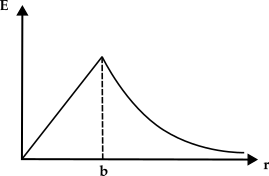
\includegraphics[width=0.38\textwidth]{images/electric_field} % Replace with your image file
\end{wrapfigure}
\begin{remark}
	Il campo $\bold{E}$ indotto esiste solo quando $\bold{B}$ \`e variabile, ossia quando le correnti non sono stazionarie. Eppure abbiamo comunque calcolato $\bold{B}(t)$ della spira usando le nozioni matematiche della magnetostatica. 
	
	I risultati ottenuti in questo modo sono tecnicamente errati, ma nella pratica restano comunque delle ottime approssimazioni quando i fenomeni sono spazialmente confinati e lentamente variabili. Ovvero si ha un approssimazione quasi statica per $\Delta x \ll c \Delta t$.
\end{remark}

\subsection{Esempio 3}

\begin{wrapfigure}{l}{0.4\textwidth}  % 'r' for right, 'l' for left
    \centering
    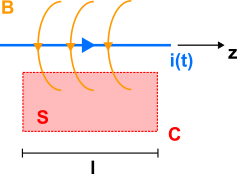
\includegraphics[width=0.38\textwidth]{images/filo_infinto} % Replace with your image file
\end{wrapfigure}
Consideriamo un filo infinito attraversato da una corrente variabile $I(t)$, il campo magnetico generato \`e
\begin{equation*}
	\bold{B}(t) = \frac{\mu_0}{2 \pi r} I(t) \bold{\hat{u}}_{\theta}
\end{equation*}
Il campo elettrico $\bold{E}$ indotto \`e ortogonale al campo magnetico $\bold{B}$, siccome si ha simmetria cilindrica $\bold{E} = E(r,t) \bold{\hat{u}}_z$.

Utilizzando la legge di Faraday in forma integrale 
\begin{equation*}
	\oint_{C} \bold{E} \cdot d \bold{l} = - \frac{d}{dt} \int_S \bold{B} \cdot d \bold{A}
\end{equation*}
preso C generico cammino rettangolare con lato maggiore di lunghezza $l$, segue che  
\begin{equation*}
	[E(r_0) - E(r)]l = - \frac{\mu_0 l}{2 \pi} \frac{d I}{dt} \int_{r_0}^{r} \frac{1}{r'}dr'
\end{equation*}
e quindi il campo elettrico ha espressione
\begin{equation*}
	\bold{E}(r) = \left(\frac{\mu_0}{2\pi}l \frac{dI}{dt} \log(r) + K\right)\bold{\hat{u}}_z
\end{equation*}
Per $r \to \infty$ il campo elettrico diverge. Il risultato ottenuto \`e corretto solo in prossimit\`a del filo. L'informazione elettromagnetica viaggia alla velocit\`a della luce e a grandi distanze $\bold{B}(t)$ non dipende dalla corrente al tempo t, ma dalla corrente ad un tempo precedente.
\newline

Se la corrente varia significativamente in un tempo caratteristico $\Delta t$, allora l'approssimazione quasistatica \`e valida solo per $\Delta x \ll c \Delta t$. 

\section{Verso le Equazioni di Maxwell}

Abbiamo visto nei capitoli precedenti e in questo come in generale le cariche siano soggette alla legge di forza 
\begin{equation*}
	\bold{F} = q ( \bold{E} + \bold{v} \times \bold{B})
\end{equation*}
dalla definizione di campo elettrico $\bold{E}$ e di campo magnetico $\bold{B}$ abbiamo derivato quatro 
leggi che legato tra loro diverse grandezze legate alla carica di un corpo:
\begin{enumerate}
	\item $\nabla \cdot \bold{E} = \frac{1}{\varepsilon_0} \rho$ \quad  \text{(Legge di Gauss):} \newline
	Tale legge dipendendo dalla carica contenuta in un volume di spazio che \`e un invariante relativistico risulta essere sempre verificata anche per cariche in moto.  
	\item $\nabla \cdot \bold{B} = 0 $:
	\newline
	Il campo magnetico \`e solenoidale e quindi il suo flusso attraverso una superficie chiusa \`e sempre nullo. Questo ci dice che non esistono cariche magnetiche elementari (monopolo).
	\item  $\nabla \times \bold{E} = - \frac{\partial \bold{B}}{\partial t}$ \quad \text{(Legge di Faraday)}:
	\newline
	La circuitazione del campo elettrico \`e pari alle variazioni nell'unit\`a di tempo di quello magnetico concatenato con il circuito. Tale legge \`e sempre verificata nel limite di campi quasistazionari. 
	\item  $\nabla \times \bold{B} = \mu_0 \bold{J}$ \quad  \text{(Legge di Amp\'ere)}
\end{enumerate}

Infine giungiamo alla legge di Amp\`ere, questa esprime la circuitazione del campo $\bold{B}$ in relazione alla corrente concatenata dal circuito moltiplicata per un fattore 
\begin{equation}
	\oint_{C} \bold{B} \cdot d\bold{l} = \mu_0 \int_{S} \bold{J} \cdot d\bold{a} = \mu_0 I
\end{equation} 
siccome il campo magnetico \`e solenoidale possiamo esprimerlo a meno di un potenziale vettore $\bold{B} = \nabla \times \bold{A}$ a patto che $\nabla \cdot \bold{A} = 0$ (gauge di Coulomb). La forma locale assume l'espressione
\begin{equation*}
	\nabla^2 \bold{A} = - \mu_0 \bold{J}
\end{equation*}
la cui soluzione ci \`e nota dai capitoli precedenti 
\begin{equation*}
	\bold{A} = \frac{\mu_0}{4 \pi} \int_{V} \frac{\bold{J}(r')}{|r-r'|}dr'
\end{equation*}
Nella forma integrale in (5.11) idealmente la superficie S pu\`o essere qualsiasi, basta che ha come contorno il circuito C per mantenere consistenza con il teorema di Stokes.  Questa relazione \`e verificata  e compatibile con l'equazione di continuit\`a (conservazione della carica elettrica) solo per fenomeni stazionari, ossia 
\begin{equation*}
	\nabla \cdot \bold{J} + \frac{\partial \rho}{\partial t}= 0
\end{equation*}
solo se $\frac{\partial \rho}{\partial t} = 0$. Dall'altronde vale anche la relazione $\nabla \cdot (\nabla \times \bold{B}) = 0$. Questo significa che un flusso che entra all'interno di un certo volume deve anche uscire, non possono esserci addensamenti di carica. Sappiamo che in generale questo non \`e sempre vero. Possiamo pensare di immagazzinare della carica in una piccola regione di spazio per poi lasciarla disperdere (scarica di un condensatore). Dato che la carica viene rilasciata dalla regione in cui era confinata, la corrente sviluppata non soddisfa la condizione di stazionariet\`a $\nabla \cdot \bold{J} = 0$, violando in questo modo la legge di Amp\'ere.

La legge di Amp\'ere richiede una generalizzazione per fenomeni non stazionari.

\begin{remark}
La legge di Faraday non presenta queste difficolt\`a, poich\`e $\nabla \cdot \bold{B} = 0$ e quindi 
\begin{equation*}
	\nabla \cdot (\nabla \times \bold{E} ) = - \frac{\partial }{\partial t}(\nabla \cdot \bold{B})= 0
\end{equation*}
\end{remark}
Nonostante non vi fosse nessuna evidenza sperimentale nell'ottocento che campi elettici $\bold{E}$ variabili inducessero campi magnetici, Maxwell not\'o l'asimettria tra le legge di Faraday e quella di Amp\'ere e si pose il problema concettuale di una generalizzazione delle equazioni del campo elettromagnetico.
\newpage

\subsection{Corrente di Spostamento}
\vspace{0.2cm}
\begin{center}
	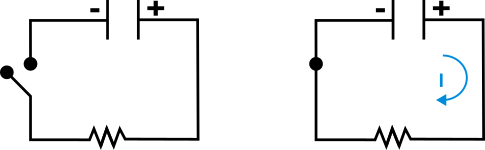
\includegraphics[width = 11.5cm]{images/transport_current}
\end{center}

Un esperimento per dimostrare la necessit\`a di una correzione della legge di Amper\'ere \`e quello della scarica e carica di un condensatore. L'idea \`e quella di di avere una configurazione in cui la corrente all'interno d i un circuito cambia nel tempo. Per farlo consideriamo un circuito RC formato da una resistenza R, un condensatore C e un interruttore. Quando chiudiamo il circuito la carica immagazzinata nel condensatore fluisce  nel circuito scaldando la resistenza.
\newline

Qual \`e il problema? Proviamo a calcolare il campo magnetico creato dalla corrente in un certo punto del circuito  usando la legge di Amp\'ere. Prendiamo una curva $\Gamma $ chiusa che racchiude il filo, con una superficie interna S. La legge di Amp\'ere in forma integrale lega il campo magnetico $\bold{B}$ alla corrente I che scorre nel circuito 
\begin{equation*}
	\int_{\Gamma} \bold{B} \cdot d \bold{r} = \mu_0 I
\end{equation*}
\begin{wrapfigure}{l}{0.4\textwidth}  % 'r' for right, 'l' for left
    \centering
    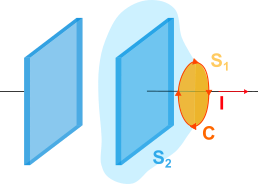
\includegraphics[width=0.38\textwidth]{images/moving_path}
\end{wrapfigure}
In questo caso la corrente I(t) cambia nel tempo.

Supponiamo di considerare una superficie $S'$ che ha sempre come contorno $\Gamma$ e si estende nella regione in cui \`e presente il condensatore. Attraverso $S'$ non passa corrente, di conseguenza se utilizziamo la legge di Amp\'ere, possiamo concludere che non ci sia campo magnetico
\begin{equation*}
	\int_{C} \bold{B} \cdot d\bold{r} = 0 
\end{equation*}
Questo porta ad avere una contraddizione con quanto determinato usando la superficie S. Il problema \`e che la legge di Amp\'ere come accennato prima risulta essere verificata solo per per correnti stazionarie che non cambiano nel tempo.
\newline

Per correggere questa limitazione della legge di Amp\'ere introduciamo un termine che prende il nome di \textit{corrente di spostamento} all'interno della sua equazione
\begin{equation}
	\nabla \times \bold{B} = \mu_0 \bold{J} + \varepsilon_0 \mu_0 \frac{\partial \bold{E}}{\partial t} 
\end{equation}
in questo modo soddisfiamo la condizione di stazionarit\`a $\nabla \cdot \bold{J} = 0$:
\begin{equation*}
	\mu_0 \left(\nabla \cdot \bold{J} + \varepsilon_0 \nabla \cdot \frac{\partial \bold{E}}{\partial t} \right)  = \nabla \cdot (\nabla \times \bold{B}) = 0
\end{equation*}
In modo simmetrico alla legge di Faraday, Maxwell propone che la circuitazione di $\bold{B}$ dipende anche dalla variazione del flusso di $\bold{E}$ concatenata con il circuito. Utilizzando la forma locale della legge di Gauss possiamo riscrivere (5.12) come:
\begin{equation}
	\nabla \cdot \bold{J} + \frac{\partial \rho}{\partial t} = 0
\end{equation}
che corrisponde all'equazione di continuit\`a che ci dice che l'elettricit\`a \`e localmente conservata. \'E solo con l'aggiunta della corrente di spostamento che l'equazione di Maxwell diventa consistente con la conservazione della carica.

La legge (5.12) come tutte le altre ammette una forma integrale 
\begin{equation}
	\oint_{C} \bold{B} \cdot d \bold{l} = \mu_0 \int_{S} \bold{J} \cdot d \bold{A} + \varepsilon_0 \mu_0 \frac{\partial }{\partial t} \int_{S} \bold{E} \cdot d \bold{A} 
\end{equation}
Riassumendo la legge di Amp\'ere-Maxwell soddisfa contemporaneamente:
\begin{enumerate}
	\item L'equazione di continuit\`a sia nel caso stazionario che non stazionario.
	\item La legge di Amp\'ere \`e ampiamente verificata su base sperimentale nel limite stazionario.
\end{enumerate}
La corrente di spostamento 
\begin{equation}
	\bold{J}_d =  \varepsilon_0 \frac{\partial \bold{E}}{\partial t}
\end{equation}
ha le dimensioni di una densit\`a di corrente. Il suo nome non indica una corrente che esiste fisicamente, ovvero nell'esempio del condensatore non si ha un reale transito di cariche tra le armature.

\subsection{Esempio: Corrente Radiale}

\begin{wrapfigure}{r}{0.4\textwidth}  % 'r' for right, 'l' for left
    \centering
    
\includegraphics[width=0.3\textwidth]{images/spheric_surface}
\end{wrapfigure}
Consideriamo un conduttore sferico con una cavit\`a al suo centro in cui \`e posta una carica Q. Nella corona sferica scorre una densit\`a di corrente $\bold{J} = \sigma \bold{E}$. Verificare la legge di Amp\'ere-Maxwell.

\begin{proof}
	La corrente che scorre sulla superficie del conduttore \`e data da
	\begin{equation*}
		I = \frac{dQ}{dt} = \int_{S} \bold{J} \cdot d \bold{A}
	\end{equation*}
Per simmetria il campo magnetico $\bold{B}$ generato dal flusso di corrente deve essere radiale. Dato che per una superficie chiusa per il campo magnetico deve valere la condizione  $\nabla \cdot \bold{B} = 0 $ e quindi 
\begin{equation*}
	\oint_{S} \bold{B}(r) \cdot d\bold{A} = B(r)4\pi r^2 = 0 \Rightarrow  \bold{B} = 0
\end{equation*}
dunque $\nabla \times \bold{B} = 0$. Dalla relazione di Amp\'ere classica abbiamo che 
\begin{equation*}
	\nabla \times \bold{B} = \mu_0 \bold{J}
\end{equation*}
ma $\bold{J} = I / 4 \pi r^2 \neq 0$ il che \`e assurdo. Di conseguenza abbiamo bisogno d'introdurre il termine della corrente di scostamento nella nostra equazione. Abbiamo che 
\begin{equation*}
	\bold{J} = - \frac{\partial Q}{\partial t} \frac{1}{4 \pi r^2} \hat{\bold{u}_{r}}
\end{equation*}
Il campo elettrico \`e 
\begin{equation*}
	\bold{E}(t) = \frac{Q(t)}{4 \pi \varepsilon_0} \frac{1}{r^2}\hat{\bold{u}}_r
\end{equation*}
e quindi la corrente di scostamento \`e 
\begin{equation*}
	\bold{J}_d = \varepsilon_0 \frac{\partial \bold{E}}{\partial t} = \frac{1}{4\pi \varepsilon_0}\frac{\partial Q}{\partial t} \bold{\hat{u}}_r = -\bold{J}
\end{equation*}
Se Q \`e positiva, $\partial Q / \partial t$ \`e negativa (la carica diminuisce), e quindi $\bold{J} >0$.
Se Q \`e negativa, $\partial Q / \partial t$ \`e positivo (la carica diminuisce in modulo, ma cambia in segno) e quindi $\bold{J} < 0$.

Utilizzando la corrente di spostamento l'equazione di Amp\`ere-Maxwell abbiamo che $\bold{B} =0 $ \`e consistente. 

\end{proof}

\subsection{Scarica del Condensatore }

\begin{wrapfigure}{l}{0.4\textwidth}  % 'r' for right, 'l' for left, width of figure
    \centering
    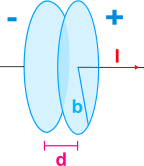
\includegraphics[width=0.24\textwidth]{images/parallel_plate} % Adjust width accordingly
\end{wrapfigure}
Ritornando all'esempio usato per introdurre l'equazione di Amp\'ere-Maxwell, abbiamo visto che senza considerare la corrente di spostamento il campo magnetico $\bold{B} = 0$ quando la superficie $S'$ attraversa il volume tra i due piatti del condensatore. La necessit\`a della corrente di spostamento ci dice che manca qualcosa alla descrizione del problema perch\`e l'accumulo di carica nei piatti del condensatore induce una dipendenza dal tempo del campo elettrico presente tra i piatti.

Nelle condizioni in cui le cariche sono statiche il campo elettrico assume l'espressione
\begin{equation*}
	\bold{E} = \frac{Q}{\varepsilon_0 A}\bold{\hat{u}}_n
\end{equation*}
dove A \`e l'area della superficie di ciascun piatto e Q la carica depositata su di essi. Si ignorando gli effetti di bordo, il che \`e accettabile se la distanza tra le armature \`e molto pi\`u piccola della loro dimensione.

 \begin{wrapfigure}{r}{0.4\textwidth}  % 'r' for right, 'l' for left, width of figure
    \centering
    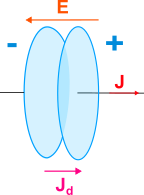
\includegraphics[width=0.24\textwidth]{images/parallel_plate1} % Adjust width accordingly
\end{wrapfigure}
 La corrente di spostamento indotta dal campo elettrico variabile 
 \begin{equation*}
 	\bold{J}_d = \frac{1}{A} \frac{dQ}{dt}
 \end{equation*}
 risulta essere parallela al campo $\bold{E}$ e discorde in verso (nella scarica il campo diminuisce e quindi $\bold{E}_{fin} < \bold{E}_{in}$), ma concorde con $\bold{J}$ nel filo. Ripetendo i calcoli per ottenere $\bold{B}$ rispetto alla superficie $S'$, dobbiamo considerare un termine in pi\`u 
 \begin{equation*}
 	\oint_{C} \bold{B} \cdot d\bold{l} = \mu_0 \left( \underbrace{\int_{S'} \bold{J} \cdot d\bold{A}}_{=0} +  \varepsilon_0 \frac{\partial }{\partial t} \int_{S'} \bold{E} \cdot d \bold{A}\right) = \mu_0 \varepsilon_0 \frac{\partial }{\partial t} \int_{S'} \bold{E} \cdot d\bold{A}
 \end{equation*}
 che possiamo riscrivere come 
 \begin{equation*}
 	B(r) 2 \pi r = \mu_0 \varepsilon_0 \frac{d \phi_E}{dt} = \mu_0 \varepsilon_0 \left(\frac{1}{\varepsilon_0 A} \frac{dQ}{dt}\right)A = \mu_0 I
 \end{equation*}
 per $\pi r^2 < S'$. Per $r>b$ dove $b$ \`e il raggio delle armature, il campo magnetico non ha discontinuit\`a e $B = \mu_0 I / 2\pi r$. Per $r<b$ si ha $S' = \pi r^2 < \pi b^2 = A$ e il campo  magnetico \`e 
 \begin{equation*}
 	B(r) 2\pi r  = \mu_0 \varepsilon_0 \left(\frac{1}{\varepsilon_0 A}\frac{dQ}{dt}\right)\pi r^2  \Rightarrow B(r) = \frac{\mu_0 I}{2 \pi b^2}r
 \end{equation*}
Il campo magnetico ha una discontinuit\`a passando attraverso le armature per $r<b$, questo \`e dovuto al fatto che la corrent $I(t)$ e i piatti si stanno scaricando. Nei piatti fluisce una corrente superficiale 

\begin{equation*}
	\Delta B_{\parallel} = \mu_0 K \Rightarrow K = \frac{1}{\mu_0}(B_{ext} - B_{in}) = \frac{I}{2\pi r}\left(1 - \frac{r^2}{b^2}\right)
\end{equation*}
In modo esplicito la corrente superficiale attraverso una circonferenza di raggio r \`e: 
\begin{equation*}
	K = \frac{I}{2 \pi r} = \frac{1}{2\pi r}\frac{dQ_r}{dt}
\end{equation*}
 \begin{wrapfigure}{l}{0.4\textwidth}
 \vspace{-1.5cm}  % 'r' for right, 'l' for left, width of figure
    \centering
    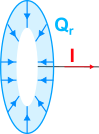
\includegraphics[width=0.23\textwidth]{images/parallel_plate2} % Adjust width accordingly
\end{wrapfigure}
dove $Q_r = Q_0\left(1-\frac{r^2}{b^2}\right)$ \`e la frazione di carica nella corona esterna di raggio r, per una distribuzione di carica uniforme. Svolgendo i conti ritroviamo quanto dedotto in precedenza dalla discontinuit\`a del campo magnetico.

\subsection{Limite Quasi-Statico}

La correzione dell'equazione di Amp\'ere da parte di Maxwell risulta trascurabile per campi lentamente variabili (quasi statici). Questa diventa significativa quando i tempi di variazione sono direttamente confrontabili con il tempo che la radiazione elettromagnetica impiega ad attraversare l'apparato. 

\subsubsection{Esempio: Condensatore con Corrente Variabile}
%IMMAGINI PAGINA 35-36 NOTE TABARELLI SETTIMANA 9%
\begin{wrapfigure}{r}{0.4\textwidth}
 % 'r' for right, 'l' for left, width of figure
    \centering
    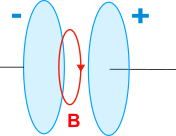
\includegraphics[width=0.3\textwidth]{images/parallel_plate3} % Adjust width accordingly
\end{wrapfigure}
Consideriamo un condensatore posto in un circuito in cui scorre una corre $I(t)$, il campo elettrico presente tra le due armature \`e dato da 
\begin{equation*}
	\bold{E} = \frac{Q(t)}{\varepsilon_0 \pi b^2}\hat{\bold{u}}_z
\end{equation*}
Il campo magnetico $\bold{B}$ indotto, prendendo un cammino $C$ con raggio $r<b$ tra le due armature \`e 
\begin{equation*}
	\bold{B}(r,t) = \frac{\mu_0 I(t)}{2 \pi b^2}r \;\hat{\bold{u}}_{\theta}
\end{equation*}
Siccome il campo magnetico risultate \`e variabile per la legge di Faraday, esiste un campo elettrico $\bold{E}_{ind}$ indotto che modifica il campo $\bold{E}(t)$ tra i due piatti
\begin{equation*}
	\nabla \times \bold{E}_{ind} = - \frac{\partial \bold{B}}{\partial t}
\end{equation*}


Per valutare la variazione del campo elettrico $\Delta E/E$ rispetto al campo elettrico del condensatore  e dato che il campo magnetico ha direzione azimutale, consideriamo un circuito C con lato maggiore $b$ raggio delle armature e lato minore dato dalla distanza $d$ tra i due piatti. Da cui calcoliamo circuitazione del campo elettrico indotto
\begin{equation*}
	\oint_{C} \bold{E}_{ind} \cdot d\bold{l} = [E(b) - E(0)]d = \Delta E_{ind}d
\end{equation*}
\begin{wrapfigure}{l}{0.4\textwidth}
 % 'r' for right, 'l' for left, width of figure
    \centering
    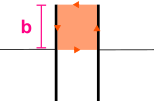
\includegraphics[width=0.3\textwidth]{images/parallel_plate4} % Adjust width accordingly
\end{wrapfigure}
analogamente deriviamo il flusso del campo magnetico attraverso la superficie racchiusa da C: 
\begin{equation*}
	\phi(\bold{B}) = \int_{0}^{d}dx \int_{0}^{b} \frac{\mu_0 I}{2 \pi b^2}r dr = \frac{\mu_0 d }{4 \pi }I
\end{equation*}
Passando dalle legge di Faraday in forma integrale abbiamo che la differenza di campo elettrico massima \`e data 
\begin{equation*}
	\Delta E_{max} = \frac{\mu_0}{4 \pi}\frac{dI}{dt}
\end{equation*}
la variazione relativa, rispetto al campo tra le due piastre \`e 
\begin{equation*}
	\frac{\Delta E_{max}}{E} = \left(\frac{\mu_0}{4 \pi} \frac{dI}{dt}\right)\left(\frac{\varepsilon_0 \pi b^2}{Q}\right)= \frac{\mu_0 \varepsilon_0}{4}b^2 \frac{1}{Q}\frac{d^2Q}{dt^2}
\end{equation*}
posta la velocit\`a della luce come $c = 1/\sqrt{\varepsilon_0 \mu_0}$  possiamo considerare due casi per calcolare esplicitamente la variazione relativa del campo:
\begin{enumerate}
	\item scarica/carica del condensatore, dove $Q(t) = Q_0 e^{-t/\tau}$ e quindi 
	\begin{equation*}
		\frac{\Delta E}{E} = \frac{1}{4} \left(\frac{b}{c \tau}\right)^2
	\end{equation*}
	\item corrente alternata, dove $Q = Q_0 \cos \left(\frac{2\pi}{T}t\right)$ e di conseguenza
	\begin{equation*}
				\frac{\Delta E}{E} = \pi^2 \left(\frac{b}{c \tau}\right)^2
	\end{equation*}
\end{enumerate}

Affinch\`e $\Delta E/E \approx1$ deve valere che $\left(\frac{b}{c \tau}\right)^2 \sim 1$. Tale condizione nel limite quasi stazionario \`e soddisfatta.

\subsubsection{Esempio: Solenoide }
%IMMAGINI PAGINA 37 NOTE TABARELLI SETTIMANA 9 %
\begin{wrapfigure}{l}{0.4\textwidth} % 'r' for right, 'l' for left
    \centering
    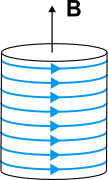
\includegraphics[width=0.18\textwidth]{images/solenoid2} % Replace with your image
\end{wrapfigure}
Consideriamo un sistema in cui \`e presente un solenoide con una densit\`a di spire $n$ attraversato da una corrente alternata $I(t) = I_0 \cos(\omega t)$. Il campo magnetico dipendente dal tempo generato \`e dato da $\bold{B}(t) = \mu_0 n I(t) \hat{\bold{u}}_z$. Determinare:
\begin{enumerate}
	\item  $E(t)$ in funzione di r;
	\item $\Delta B(t)$ dovuto a $E(t)$;
	\item Mostrare che $\Delta B /B \ll 1$ per fenomeni quasi statici.
\end{enumerate}



1)  Campo elettrico e magnetico variabile sono legati tra loro dalla legge di Faraday
\begin{equation*}
	\nabla \times \bold{E} = - \frac{\partial \bold{B}}{\partial t}
\end{equation*}
\begin{wrapfigure}{r}{0.4\textwidth} % 'r' for right, 'l' for left
    \centering
    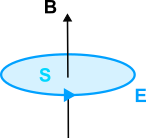
\includegraphics[width=0.3\textwidth]{images/circular_path} % Replace with your image
\end{wrapfigure}
siccome il campo magnetico ha direzione assiale, il campo elettrico indotto deve avere direzione azimutale, ed \`e costante per $r$ fissato. Per la simmetria del problema prendiamo un cammino circolare di raggio $r$ che circonda il solenoide. Passando alla forma integrale della legge di Faraday
\begin{equation*}
	\oint_{C} \bold{E} \cdot d \bold{l} = - \frac{\partial}{\partial t} \int_{S} \bold{B} \cdot d\bold{A}
\end{equation*} 
Siccome $B(t)$ \`e uniforme abbiamo che 

\begin{equation*}
	E(r)2 \pi r = - \frac{d}{dt}(B \pi r^2) \Rightarrow E(r) = -\frac{1}{2}\mu_0 n r \frac{dI}{dt}
\end{equation*}
\begin{wrapfigure}{l}{0.4\textwidth} % 'r' for right, 'l' for left
    \centering
    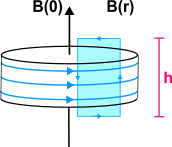
\includegraphics[width=0.3\textwidth]{images/circular_path1} % Replace with your image
\end{wrapfigure}

2) Prendendo un cammino rettangolare  C interno al solenoide con altezza $h$ e ampiezza $r$, utilizzando la legge di Maxwell, calcoliamo
\begin{equation*}
	\oint_{C} \bold{B} \cdot d \bold{l} = [B(r) - B(0)]h = \Delta B h
\end{equation*}  
e 
\begin{equation*}
	\int_{S} \bold{E} \cdot d\bold{A} = \int_{0}^{h}dz \int_{0}^{r} \frac{1}{2}\mu_0 n r \left(\frac{dI}{dt}\right)dr = \mu_0 n h \frac{r^2}{4}\frac{dI}{dt} 
\end{equation*}
mettendo insieme 
\begin{equation*}
	\Delta B = \mu_0 \varepsilon_0 \frac{\partial \phi_{S}(E)}{\partial t} = \mu_0 \varepsilon_0 \left(\mu_0 n \frac{r^2}{4}\right) \frac{d^2I}{dt^2}
\end{equation*}
3) La variazione relativa \`e data da 
\begin{equation*}
	\frac{\Delta B}{B} = \frac{mu_0 \varepsilon_0}{4} \frac{r^2}{I} \frac{d^2I}{dt^2}
\end{equation*}
Analogamente al caso del condensatore il termine 
\begin{align*}
	\frac{1}{I}\frac{d^2I}{dt^2} = \left \{ \begin{array}{l}
		\omega^2 = \left(\frac{2\pi}{T}\right)^2 \quad \text{corrente alternata} \\ \rule{0pt}{20pt}
		\frac{1}{\tau^2} \quad \text{scarica / carica di un condensatore}
	\end{array}\right.
\end{align*}
e le rispettiva variazioni relative sono date da 
\begin{equation*}
	\frac{\Delta B}{B} = \frac{1}{4} \left(\frac{r}{c \tau}\right) \quad \text{o} \quad \frac{\Delta B}{B} = \pi^2 \left(\frac{r}{c \tau}\right)^2
\end{equation*} 
affinch\`e si abbia il limite quasi stazionario $r/c\tau \sim 1$, ovvero $c \tau \sim 1$. 
Se consideriamo numericamente $c = 3 \times 10^8$ e $r = 3 - 30\;cm$, abbiamo che $\tau \sim 10^{-9} -10^{-10}$ si ottiene una correzione dell' $1 \%$ per $1/\tau = 10^7/10^8 Hz$.

Tutti i risultati "statici" restano validi fino a frequenze relativamente elevate.
 


\section{Induzione Elettromagnetica }

In questa sezione  ricaviamo alcune propriet\`a della legge di Faraday che ne semplificano l'applicazione nell'analisi di configurazioni con circuiti, in cui il campo $\bold{E}$ indotto, si manifesta sul circuito come una forza elettromotrice:
\begin{equation*}
	\oint_{C} \bold{E} \cdot d \bold{l} = - \frac{d}{dt} \int_{S} \bold{B} \cdot d \bold{A}
\end{equation*}
 
 \subsection{Mutua Induttanza}
 
 Dati due circuiti $C_1$ e $C_2$ in posizioni relative fisse, si fa scorre una corrente variabile $I_1 $ nel primo. Il flusso del campo magnetico $\bold{B}_1$ indotto, attraversa la superficie $S_2$ racchiusa in dal circuito $C_2$. Il flusso di $\bold{B}_1$
 \begin{equation*}
 	\phi_{21} (\bold{B}_1) = \int_{S_2}\bold{B}_1 \cdot d\bold{A} 
 \end{equation*}
 \`e proporzionale a $I_1$ e dipende dalla geometria del circuito. Per vedere la proporzionalit\`a a $I_1$ \`e sufficiente applicare la legge di Biot-Savart:
 \begin{equation*}
 	\bold{B}_1(\bold{r}) = \frac{\mu_0}{4 \pi}I_1 \oint_{C_1} \frac{d\bold{l} \times \hat{\bold{u}}_z}{|\bold{r} - \bold{r}'|^2}
 \end{equation*}
come conseguenza si ha il flusso di $\bold{B}_1$ attraverso $C_2$ \`e a sua volta proporzionale alla corrente $I_1$:
\begin{equation*}
	\phi_{21}  = \int_{S_2}\bold{B}_1 \cdot d \bold{A} = \frac{\mu_0}{4 \pi}I_1 \int_{S_2} \left(\oint_{C_1} \frac{d \bold{l} \times \bold{\hat{u}}_r}{|\bold{r} - \bold{r}'|^2}\right) \cdot d \bold{A} = M_{21}I_1
\end{equation*}
dove il termine $M_{21}$ racchiude la geometria del problema.

Se $I_1(t)$ cambia abbastanza lentamente, ossia con un tempo molto pi\`u grande di quello che i campi impiegano a propagarsi su $C_1$, $C_2$ e da $C_1$ a $C_2$, la forza elettromotrice indotta su $C_2$ \`e data da:
\begin{equation}
	\mathcal{E}_{21} = - \frac{d\phi_{21}}{dt} = -M_{21} \frac{dI_1}{dt}
\end{equation}
La costante $M_{21}$ prende il nome di \textit{mutua induttanza} ed \`e l'equivalente magnetico dei coefficienti di induzione (di potenziale) in elettrostatica. Tale costante mette in relazione la forza elettromotrice in un circuito con la variazione di corrente in un altro circuito.
\newline

La sua unit\`a di misura nel sistema internazionale \`e \textit{l'henry}
\begin{equation*}
	[M] = \frac{[Volt][Rempo]}{[Ampere]} = henry
\end{equation*}

\subsubsection{Esempio: Anelli Concatenati e Complanari}
%IMMAGINE PAGINA 4 SETTIMANA 10 TAABARELLI%

Consideriamo due anelli innestati l'uno dentro l'altro in modo che siano complanari dove il primo ha un raggio $R_2 \ll R_1$ del secondo. Il campo $\bold{B}_1$ relativo al circuito pi\`u grande e dovuto ad una corrente $I_1$, \`e uniforme sulla superficie di racchiusa dall'anello $C_2$.

Al centro della spira circolare il campo magnetico vale 
\begin{equation*}
	\bold{B}_1(0,0,0) = \frac{\mu_0 I_1 }{2 R_1}
\end{equation*}
e il corrispettivo flusso 
\begin{equation*}
	\phi_{21} = \int_{S_2} \bold{B}_1(\bold{r}) \cdot d\bold{A} \simeq B_{1}(0,0,0)\pi R_2^2 = \frac{\mu_0 \pi R_2^2}{2 R_1}I_1
\end{equation*}
Di conseguenza il termine di mutua induttanza \`e dato da 
\begin{equation*}
	M_{21} = \frac{\phi_{21}}{I_{1}} = \frac{\mu_0 \pi R_2^2}{2 R_1}
\end{equation*}
e quindi la forza elettromotrice indotta \`e parti a 
\begin{equation*}
	\mathcal{E}_{21} = - M_{21} \frac{d\phi_{21}}{dt} = -\frac{\mu_0 \pi R_2^2}{2R_1}\frac{dI_1}{dt}
\end{equation*}
Dalla regola di Lenz  sappiamo che se la corrente $I_2$ indotta in $C_2$ genera un campo $\bold{B}_2$, il flusso di quest'ultimo deve contrastare la variazione di flusso di $\bold{B}_1$ e quindi $\Delta \bold{B}_{2}$ \`e opposto in verso a $\Delta \bold{B}_1$. Se $I_1$ aumenta in senso orario allora $I_2$ aumenta in senso antiorario.

\subsubsection{Bobine}
%IMMAGINE %
Aumentando gli avvolgimenti, si pu\`o aumentare la mutua induttanza. Se consideriamo $N_1$ avvolgimenti sottili su $C_1$ allora $\bold{B}_{1}^{tot} = \sum_{i=1}^{N_1}\bold{B}_i = N_1 \bold{B}_{1}$. Mentre per $N_2$ avvolgimenti su $C_2$ si ha $\phi_{21}^{tot}(\bold{B}_1^{tot}) = N_2 \phi_{21}(\bold{B}_1^{tot})$ e quindi 
\begin{equation*}
	\phi_{21} = \left( \frac{\mu_0 I}{2R_1}N_1 \right)\left(N_2 \pi R_2^2\right)
\end{equation*}
il coefficiente di mutua induttanza \`e dunque dato da 

\begin{equation*}
	M_{21} = \frac{\phi_{21}}{I} = \frac{\mu_0 \pi}{2}N_1N_2\frac{R_2^2}{R_1}
\end{equation*}

\subsubsection{Caso Generale}

In situazioni in cui la geometria del problema non \`e ben definita (o in tutti i casi reali non idealizzati) la mutua induttanza pu\`o essere caratterizzata per via sperimentale 
\begin{equation}
	M_{21} \equiv  - \frac{\mathcal{E}_{21}}{dI/dt}
\end{equation}

\subsubsection{Teorema di Reciprocit\`a della Mutua Induttanza}

%IMMAGINE PAGINA 6 SETTIMANA 10%

Per ogni coppia di circuiti $C_1$ e $C_2$ fissati relativamente tra loro e in cui \`e possibile far scorrere una corrente, i rispettive coefficienti di mutua induttanza sono
\begin{equation*}
	M_{21} = \frac{\phi_{21}}{I_1} \quad \text{e} \quad M_{12} = \frac{\phi_{12}}{I_2}
\end{equation*}
e vale l'uguaglianza 
\begin{equation}
	M_{21} = M_{12}
\end{equation}
Tale relazione vale per una qualsiasi coppia di circuiti e non richiede simmetrie geometriche.

\begin{proof}
Utilizziamo il potenziale vettore $\bold{A}$ per il calcolo del flusso di $\bold{B}$ abbiamo
\begin{equation*}
	\int_{S}\bold{B} \cdot d\bold{a} = \int_{S}(\nabla \times \bold{A}) \cdot d\bold{a} = \oint_{C} \bold{A} \cdot d\bold{l}
\end{equation*}	
In questo modo possiamo calcolare il flusso tramite l'integrale di linea di $\bold{A}$.

Il potenziale $\bold{A}_{21}$, dovuto alla corrente $I_1$ nel circuito $C_1$, sull'elemento d$\bold{l}_2$ \`e dato da:
\begin{equation*}
	\bold{A}_{21}= \frac{\mu_0 }{4 \pi}	I_1 \oint_{C_1}\frac{d \bold{l}_1}{r_{21}}
\end{equation*} 
Il flusso di $\bold{B}_1$ concatenato al circuito $C_1$ \`e:
\begin{align*}
	\phi_{21} & = \oint_{C_2} \bold{A}_{21} \cdot d\bold{l}_2 = \frac{\mu_0}{4 \pi}I_1 \oint_{C_2}\left[\oint_{C_1} \frac{1}{r_{21}}d\bold{l}_1 \right] \cdot d\bold{l}_2 = \\ \rule{0pt}{15pt}
	& = \frac{\mu_0}{4 \pi}I_1 \oint_{C_2} \oint_{C_1} \frac{d \bold{l}_1 \cdot d\bold{l}_2}{r_{21}}
\end{align*}
In modo analogo scambiando i ruoli di $C_1$ e $C_2$ definiamo
\begin{equation*}
	\phi_{12} = \frac{\mu_0}{4 \pi}I_2 \oint_{C_1}\oint_{C_2} \frac{d \bold{l}_2 \cdot \bold{l}_1}{r_{12}}
\end{equation*}
Gli integrali contengono la geometria del sistema:
\begin{enumerate}
	\item $r_{12} = |\bold{r_{12}}| = |\bold{r}_{21}| = r_{21}$;
	\item $d \bold{l}_1 \cdot d \bold{l}_2 = d \bold{l}_2 \cdot d\bold{l}_1$;
	\item l'ordine di integrazione significa che si sommano gli stessi termini con ordine differente.
\end{enumerate}
Possiamo concludere che 
\begin{equation*}
	M_{21} = \frac{\phi_{21}}{I_1} = \frac{\phi_{12}}{I_2} = M_{12}
\end{equation*}

\end{proof}

\subsubsection{Esempio: Bobine Concentriche e Complanari}

%IMMAGINE PAGINA 7 SETTIMANA 10%

Consideriamo una bobina $C_1$ di raggio $R_1$ con $N_1$ avvolgimenti e resistenza R, al suo inerno \`e presente una seconda bobina con $N_2$ avvolgimenti e raggio $R_2 \ll R_1$. Quest'ultima \`e collegata a una batteria che fa scorrere una corrente $I_2$ al suo interno.
\newline

La corrente indotta in $C_1$ \`e data da 
\begin{equation*}
	I_1 = \frac{\mathcal{E}_{12}}{R} = - \frac{1}{R} \frac{d\phi_{12}}{dt} = -\frac{1}{R}M_{12} \frac{dI_2}{dt}
\end{equation*}
Il coefficiente di mutua induttanza $M_{12}$ non \`e calcolabile in modo immediato perch\`e $\bold{B}_2$ dovuto alla corrente $I_2$, non \`e uniforme sulla superficie $S_1$ delimitata da $C_1$. Per\`o abbiamo visto nell'esempio precedente che \`e possibile calcolare $M_{21}$ e usando il teorema di reciproca induttanza otteniamo $M_{12}$.

\subsection{Autoinduttanza}

%IMMAGINE PAGINA 8 SETTIMANA 10%

Una corrente I fluisce all'interno di un circuito C, se questa \`e variabile di conseguenza anche il campo $\bold{B}$ cambia e quindi anche il suo flusso attraverso la superficie S racchiusa da C:
\begin{equation*}
	\phi = \int_{S} \bold{B} \cdot d \bold{a} = \frac{\mu_0}{4 \pi}I \int_{S}\left(\oint_{C} \frac{d \bold{l} \cdot \bold{\hat{u}}_{r}}{r^2}\right) \cdot d \bold{a}
\end{equation*}
Il flusso \`e proporzionale alla corrente per fattori che dipendono dalla geometria del problema.  Si definisce $autoinduttanza$ (o $induttanza$) la grandezza 
\begin{equation}
	L = \frac{\phi}{I}
\end{equation} 
Poich\`e la legge di Faraday vale qualunque origine abbia la variazione di flusso, abbiamo una forza elettromotrice autoindotta
\begin{equation*}
	\mathcal{E} = - \frac{d\phi}{dt}
\end{equation*}
che si oppone alla variazione di flusso in , ossia oppone resistenza all'instaurarsi della corrente I. Dalla relazione (5.19) possiamo legare induttanza e forza elettromotrice 
\begin{equation}
	\mathcal{E} = - L \frac{dI}{dt}
\end{equation}

\begin{remark}
	La forza elettromotrice e il campo $\bold{B}$ sono legati da una relazione locale $\nabla \times \bold{E} = - \partial \bold{B}/\partial t$, che non dipende dalla natura delle sorgenti.
\end{remark}

\subsubsection{Esempio: Induttanza per una Bobina Circolare}
%IMMAGINI PAGINA 9 SETTIMANA 10%

Data una bobina toroidale di altezza $h$ con raggio interno $a$, raggio esterno $b$ dotata di N avvolgimenti, calcolare la sua autoinduttanza.

\begin{proof}
	Dalla legge di Amp\'ere in coordinate cilindriche, calcoliamo il campo magnetico:
	\begin{align*}
		\bold{B}(r) = \left \{ \begin{array}{l}
			\frac{\mu_0 N I}{2 \pi r}\bold{\hat{u}}_{\theta} \quad r \in [a,b], \; z\in \left[-\frac{h}{2},\frac{h}{2} \right] \\ \rule{0pt}{20pt}
			0 \quad \text{altrove}
		\end{array}\right.
	\end{align*}
Il flusso concatenato da una spira \`e dato da 
\begin{equation*}
	\phi_{A}(\bold{B}) = \frac{\mu_0I}{2 \pi}h \int_{a}^{b} \frac{1}{r}dr = \frac{\mu_0  I}{2 \pi}h \log\left(\frac{b}{a}\right)
\end{equation*}	
e quindi il flusso totale concatenato dal solenoide \`e dato da 
\begin{equation*}
	\phi_{tot}(\bold{B}) = N \phi_{A}(\bold{B})
\end{equation*}

\end{proof} 

In generale se la geometria del problema non \`e nota, L \`e misurabile.

\section{Induttanza come Elemento Circuitale (Circuito RL)}

%IMMAGINE QUI PAGINA 10 SETTIMANA 10%

Dato un circuito formato da una batteria (forza elettromotrice), una resistenza R, un induttanza L e un interruttore che permette di chiudere il circuito. Sperimentalmente possiamo riprodurre il circuito pensandolo come ad una batteria collegata da una bobina formata da un filo conduttore con resistenza R.
\newline

Al fluire di una corrente I, utilizzando la legge delle maglie (seconda legge di Kirchoff), dobbiamo avere che la somma algebrica delle tensioni lungo una maglia chiusa deve essere nulla, e quindi 
\begin{equation}
	\mathcal{E}_0 + \mathcal{E}_{L} = RI \quad \Rightarrow \quad \mathcal{E}_0 = L\frac{d I}{dt} + RI
\end{equation}
dove con $\mathcal{E}_0$ indichiamo la forza elettromotrice fornita dalla batteria (tensione), mentre $\mathcal{E}_L$ \`e la $fem$ indotta in un induttanza ideale. Anche in questo caso possiamo identificare $\mathcal{E}_L$ come la differenza di potenziale ai capi di L.
$\mathcal{E}_L$ \`e negativa perch\`e si oppone al passaggio di corrente all'interno dell'induttanza. Per correnti stazionarie ($\mathcal{E}_L = 0$) e il circuito \`e puramente resistivo.
\newline

Se consideriamo correnti variabili $I(t)$ all'interno del circuito, dove al tempo $t<0$ l'interruttore \`e aperto e la corrente vale $I(0) = 0$, per $t \geq 0$ l'interruttore \`e chiuso e quindi $I =I(t)$. Nell'ultimo caso l'equazione (5.21) \`e un equazione differenziale lineare non omogenea del primo grado:
\begin{equation*}
	L \frac{dI}{dt} + RI = \mathcal{E}_0
\end{equation*}
la sua soluzione \`e
\begin{equation}
	I(t) = \frac{\mathcal{E}_0}{R} + A e^{-\frac{R}{L}t}
\end{equation} 
imponendo la condizione iniziale $I(0)=0$ si ha che la costante $A = - \mathcal{E}_0/R$ e quindi (5.22) diventa 
\begin{equation}
	I(t) = \frac{\mathcal{E}_0}{R}\left(1-e^{\frac{R}{L}t}\right)
\end{equation}
definiamo $\tau = \frac{L}{R}$, che determina la velocit\`a di transizione in cui la corrente si stabilizza intorno al valore stazionario $\mathcal{E}_0/R$ e la tensione sull'induttore diventa zero. Il tempo di transizione \`e dovuto al fatto che la carica non \`e istantanea, la bobina  si oppone all'instaurarsi della corrente e $\mathcal{E}_L$ si oppone alla variazione di flusso (legge di Lenz).

Il tempo di stabilizzazione (transiente) dipende da L, maggiore \'e il suo valore e pi\`u lento  \`e il transitorio. Se $\mathcal{E}_0 = 0$ allora $I(t) = 0$, non possono esserci correnti autoindotte senza l'immissione di lavoro esterno, perch\`e $\mathcal{E}_{L}$ si oppone alle variazioni di flusso.

\subsection{Scarica di un Induttore}

%IMMAGINE PAGINA 12 SETTIMANA 10 %

Si ha un circuito RL la cui condizione iniziale sulla corrente \`e data da $I(t) = \mathcal{E}_0/R$, al tempo $t = 0$ l'interruttore posto all'interno del circuito esclude la batteria e chiude l'induttanza L su R con un filo (corto-circuito).

\begin{remark}
Aprire un induttore senza cortocircuitare i capi non \`e prudente (se L \`e grande). L'induttore si oppone cambi di flusso di $\bold{B}$ e vuole mantenere la corrente, di conseguenza si ha una scarica elettrica. 	
\end{remark}

L'equazione per la corrente al tempo $t \geq 0$ \`e:
\begin{equation*}
	L \frac{dI}{dt} + RI = 0
\end{equation*}
la cui soluzione \`e data da
\begin{equation*}
	I(t) = I_0 e^{- \frac{R}{L}t}
\end{equation*}
dove la costante $I_0 = \mathcal{E}_0 / R$ \`e fissata dalla condizione iniziale e quindi
\begin{equation}
	I(t) = \frac{\mathcal{E}_0}{R}e^{- \frac{R}{L}t}
\end{equation} 
il transiente della scarica ha le stesse costanti di tempo della carica. Per un tempo $t \gg \tau $ si raggiunge il regime stazionario in cui I=0. Non sono presenti correnti auto indotte senza immissione di lavoro esterno. L'induttanza \`e un componente passivo (come resistenze e condensatori), non richiede lavoro meccanico o chimico/termico come un generatore.

\subsection{Combinazione di Induttori}

Dato un un circuito con pi\`u induttori attraversati da una corrente I, definiamo la forza elettromotrice della prima componente come 
\begin{equation*}
	\mathcal{E}_1 = - L_1 \frac{dI_1}{dt}
\end{equation*}
e definiamo la loro mutua induttanza come 
\begin{equation*}
	\mathcal{E}_j = -M_{1j} \frac{d I_j}{dt} 
\end{equation*}
La forza elettromotrice \`e una grandezza additiva per il principio di sovrapposizione
\begin{align}
	\mathcal{E}_i &= - \frac{d\phi}{dt} = - \frac{d}{dt} \int_{S} \bold{B} \cdot d\bold{a} = - \frac{d}{dt} \int_{S_i} (\bold{B}_{1} + \bold{B}_{2} + ...+ \bold{B}_{N}) \cdot d \bold{a} = \notag \\ \rule{0pt}{20pt} 
	& = - \frac{d}{dt}(\phi_1 + ....+ \phi_N) = -L_{i} \frac{dI_i}{dt} - \sum_{i \neq j}M_{ij}\frac{dI_j}{dt}
\end{align}
dunque la tensione ai capi dell'induttore i-esimo \`e 
\begin{equation}
	V_i = L_i \frac{d I_i}{dt} + \sum_{i \neq j} M_{ij}\frac{dI_j}{dt}
\end{equation}

\subsubsection{Induttori in Serie}

%IMMAGINE PAGINA 13 SETTIMANA 10%

Preso un circuito ideale ( in cui R = 0) formate da due induttanze in successione e attraversato da una corrente I generata da una batteria $\mathcal{E}$. La tensione sui singoli induttori \`e differente, di conseguenza la tensione totale \`e data da 
\begin{equation*}
	V = V_1 + V_2 = (L_1 + L_2) \frac{dI}{dt} + 2M \frac{dI}{dt} = (L_1 + L_2 + 2M) \frac{dI}{dt}
\end{equation*}
e quindi possiamo ricondurre il circuito ad un induttanza equivalente data da
\begin{equation}
	L = L_1 + L_2 + 2M
\end{equation}
Se $M_{ij} \ll L_i$ possiamo considerare solo $L = \sum_{i} L_i$.

\subsubsection{Induttori in Parallelo}
%IMMAGINE QUI%

Consideriamo un circuito ideale (R = 0) in cui sono presenti due induttori in parallelo, attraversati da una corrente I data da un generatore $\mathcal{E}$.  La tensione sulle singole induttanze \`e la medesima 
\begin{align*}
	\mathcal{E} = L_1 \frac{d I_1}{dt} + M \frac{dI_2}{dt} \\ \rule{0pt}{30pt} 
	\mathcal{E} = L_2 \frac{d I_2}{dt} + M \frac{d I_1}{dt}
\end{align*}
La corrente si biforca nei due rami: 
\begin{equation*}
	\frac{dI}{dt} = \frac{d I_1}{dt} + \frac{dI_2}{dt}
\end{equation*}
Isoliamo rispetto a $dI_1/dt$ e $dI_2/dt$ le due equazioni di partenza
\begin{align*}
	\mathcal{E}  = (L_1 -M) \frac{d I_1}{dt} + M \frac{d I}{dt} \quad \Rightarrow \quad \frac{d I_1}{dt} = \frac{1}{L_1-M} \mathcal{E} - \frac{M}{L_1-M} \frac{d I}{dt} \\ \rule{0pt}{30pt}
	\mathcal{E}  = (L_2 - M) \frac{d I_2}{dt} + M\frac{dI}{dt} \quad \Rightarrow \quad \frac{dI_2}{dt} = \frac{1}{L_2 - M} \mathcal{E} - \frac{M}{L_2 - M} \frac{d I}{dt}
\end{align*}
sostituendo nell'equazione della corrente 
\begin{equation*}
	\frac{dI}{dt} \left( 1 + \frac{M}{L_1 - M} + \frac{M}{L_2 -M}\right) = \left( \frac{1}{L_1 - M} + \frac{1}{L_2-M} \right)\mathcal{E}
\end{equation*}
facendo denominatore comune e riorganizzando i termini, si trova:

\begin{equation*}
	\mathcal{E} = \left( \frac{L_1L_2 - M^2}{L_1 + L_2 - 2M}\right)\frac{dI}{dt}
\end{equation*}
Dunque l'induttanza equivalente \`e:

\begin{equation}
	L = \frac{L_1 L_2 - M^2}{L_1 + L_2 -2M}
\end{equation}
Nel limite in cui $M \to 0$ e le induttanze risultano essere trascurabili abbiamo che 
\begin{equation*}
	L = \frac{L_1L_2}{L_1 + L_2} = \frac{1}{L_1} + \frac{1}{L_2}
\end{equation*}
dunque in generale 
\begin{equation}
	L = \sum_i \frac{1}{L_i}
\end{equation}

\subsection{Trasformatore}

%IMMAGINE QUI PAGINA 14 SETTIMANA 10%
Un trasformatore \`e costituito da due bobine solenoidali lineari, con stessa sezione S e lunghezza $l$, date da $N_1$ e $N_2$ avvolgimenti nel circuito primario e secondario. Ipotizzando che il campo magnetico nei solenoidi sia uniforme e che il campo disperso (ossia il campo all'esterno del solenoide) sia nullo. 
\newline

Per un trasformatore ideale il flusso passa attraverso tutti gli avvolgimenti delle bobine, facendo passare della corrente alternata nel primo circuito otteniamo una forza elettromotrice $\mathcal{E}_1 = \mathcal{E}_1(t)$, mentre nel secondo compare una forza elettromotrice indotta $\mathcal{E} = \mathcal{E}_2(t)$.

Si pu\`o regolare la tensione in uscita tramite il rapporto del numero di avvolgimenti:
\begin{equation*}
	V_2 = \frac{d\phi_2}{dt}(\bold{B}) = N_2 \frac{d \phi_{anello}(\bold{B})}{dt} = \frac{N_2}{N_1} \frac{N_1d \phi_{anello}(\bold{B})}{dt} = \frac{N_2}{N_1} \frac{d \phi_1(\bold{B})}{dt} = \frac{N_2}{N_1} \mathcal{E}_1
\end{equation*}
Per $N_2 > N_1$, la tensione in uscita \`e maggiore della tensione in ingresso. 

La conservazione dell'energia non \`e violata, perch\`e la potenza di uscita sul secondo circuito $C_2$  e di ingresso sul primo $C_1$ sono identiche (nel limite ideale):
\begin{equation*}
	\langle P_{in} \rangle = \langle \mathcal{E}_1 I_1 \rangle = \langle \mathcal{E}_2 I_2 \rangle = \langle P_{out} \rangle 
\end{equation*}

\begin{proof}
Ciascun solenoide gode dell seguenti propriet\`a:
\begin{enumerate}
	\item auto-induttanza:
	\begin{equation*}
		L_i = \mu_0 \frac{S}{l}N_i^2
	\end{equation*}
	\item mutua induttanza tra solenoide:
	\begin{equation*}
		M_{ij} = \mu_0 \frac{S}{l}N_i N_j
	\end{equation*}
\end{enumerate}
Nell'ipotesi di solenoide ideale, il campo \`e assiale e uniforme sulla sua sezione $\bold{S} = S \hat{\bold{u}}_z$.
\begin{equation*}
	\bold{B}_l = \mu_0 \frac{N_i}{l}I \hat{\bold{u}}_z
\end{equation*}
Il flusso totale \`e $N_i$ volte il flusso attraverso una singola spira:
\begin{align*}
	& L_i = \frac{\phi_i(\bold{B}_i)}{I} = N_i \frac{\phi_{i,spira}(\bold{B}_i)}{I} = \mu_0 \frac{N_i^2}{l}\hat{\bold{u}}_z \cdot S \hat{\bold{u}}_z = \mu_{0} \frac{S}{l}N_i^2 \\ \rule{0pt}{30pt}
	& M_{ij} = \frac{\phi_i(\bold{B}_j)}{I} = N_i \frac{\phi_{i,spira}(\bold{B}_j)}{I} = \mu_0 \frac{N_i N_j}{l} \hat{u}_z \cdot S \hat{u}_z = \mu_0\frac{S}{l}N_iN_j
\end{align*}
ne consegue che $M_{ij} = \sqrt{L_i L_j}$
\newline

Le equazioni del circuito sono date dalle leggi di Kirchoff su due maglie accoppiate, ma indipendenti:
\begin{equation*}
\left \{ \begin{array}{l}
	 \mathcal{E}_1 =  L_1 \frac{d I_1}{dt} + M \frac{d I_2}{dt} \\ \rule{0pt}{25pt}
	L_2 \frac{d I_2}{dt} + M \frac{d I_1}{dt} = -RI_2
	\end{array}\right .
\end{equation*}
risolvendo per esplicitare  $I_1$ e $I_2$:
\begin{equation*}
\left \{ \begin{array}{l}
	\frac{d I_1}{dt} = - \frac{1}{M} \left( RI_2 + L_2 \frac{dI_2}{dt}\right) \\ \rule{0pt}{25pt}
	\mathcal{E}_1 = - \frac{L_1}{M}R I_2 - \frac{L_1 L_2}{M} \frac{d I_2}{dt} + M \frac{d I_2}{dt}
\end{array}\right.
\end{equation*} 
siccome $M^2 = L_1 L_2$ dal risultato trovato, abbiamo che 
\begin{equation*}
	\left \{ \begin{array}{l}
		I_2 = - \frac{1}{R} \sqrt{\frac{L_2}{L_1}}\mathcal{E}_1 \\ \rule{0pt}{25pt}
		I_1 =  \frac{1}{R}\frac{L_2}{L_1} \mathcal{E}_1 + \frac{1}{L_1} \int \mathcal{E}_1 dt
	\end{array}\right .
\end{equation*}
Siccome per ipotesi il circuito \`e alimentato con della corrente alternata $\mathcal{E}_1 = V_0 \cos(\omega t)$, abbiamo che la potenza media in ingresso \`e 
\begin{equation*}
	\langle P_{in}\rangle = \langle \mathcal{E}_1 I_1 \rangle = \frac{1}{R} \frac{L_2}{L_1} \langle \mathcal{E}_1^2 \rangle + \frac{1}{L_1} \langle \mathcal{E}_1 \int \mathcal{E}_1 dt \rangle = \frac{1}{2} \frac{1}{R}\frac{L_2}{L_1}V_0 ^2 = \langle R I_2^2 \rangle  = \langle P_{out} \rangle
\end{equation*}
dove il termine $\frac{1}{L_1} \langle \mathcal{E}_1 \int \mathcal{E}_1 dt \rangle \sim \langle \sin(\omega t) \cos(\omega t) \rangle = 0$.

\end{proof}

\textbf{Corollario:} $I_2/I_1 = \mathcal{E}_{1} / \mathcal{E}_2$ se $\mathcal{E}_2 \gg \mathcal{E}_1$ e $I_2 \ll I_1$.

\section{Energia Magnetica}

La definizione dell'induttanza \`e utile per ricavare l'energia immagazzinata nel campo magnetico. Dato un circuito C attraversato da una corrente I. La forza elettromotrice indotta \`e
\begin{equation*}
	\mathcal{E} =  - \frac{d \phi}{dt} = -L \frac{dI}{dt}
\end{equation*} 
La forza elettromotrice come definita in precedenza pu\`o essere pensata come il lavoro necessario a muovere un unit\`a di carica lungo il circuito. Data una corrente I, in un tempo $dt$, viene spostata una quantit\`a di carica $Idt$ all'interno del circuito e il lavoro svolto \`e 
\begin{equation*}
	dW = \mathcal{E}Idt=-L I \frac{dI}{dt}dt \quad \Rightarrow \quad \frac{dW}{dt} = -LI \frac{dI}{dt} = -\frac{1}{2}\frac{d I^2}{dt}
\end{equation*}
Il lavoro necessario a far fluire la corrente nel circuito \`e uguale e contrario. Integrando rispetto al tempo, per un circuito C con induttanza L si ha un lavoro totale 
\begin{equation}
	U = W = \frac{1}{2}L I^2 = \frac{1}{2}I \phi
\end{equation}
Analogamente a quanto discusso per l'energia del campo elettrico identifichiamo l'energia immagazzinata nel sistema con U. Possiamo scrivere (5.30) esplicitamente rispetto al campo magnetico
\begin{equation*}
	U = \frac{1}{2} I \int_{S} \bold{B} \cdot d\bold{S} = \frac{1}{2}I \int_{S} (\nabla \times \bold{A}) \cdot d\bold{S} = \frac{1}{2}I \oint_{C} \bold{A} \cdot d \bold{r} = \frac{1}{2} \int d^3x \;\bold{J} \cdot \bold{A}
\end{equation*} 
dove nell'ultima uguaglianza si \`e usato il risultato in cui la densit\`a di corrente $\bold{J}$ \`e localizzata lungo la curva C per riscrivere l'integrale in uno rispetto allo spazio. Utilizzando l'equazione di Maxwell $\nabla \times \bold{B} = \mu_0 \bold{J}$ possiamo riscrivere l'energia come 
\begin{equation*}
	U = \frac{1}{2 \mu_0} \int d^3x \; (\nabla \times \bold{B}) \cdot \bold{A} = \frac{1}{2 \mu_0} \int_{V} d^3x \; [\nabla \cdot (\bold{B} \times \bold{A} ) + \bold{B} \cdot (\nabla \times \bold{A})]
\end{equation*}
dove l'ultimo termine \`e dovuto alle propriet\`a dell'operatore gradiente. Assumendo che $\bold{B}$ e $\bold{A}$ decrescano in modo sufficientemente veloce ad infinito, possiamo considerare il primo addendo nullo e quindi otteniamo una seconda espressione dell'energia equivalente alla prima 
\begin{equation}
	U = \frac{1}{2 \mu_0} \int_{V} d^3 x \; \bold{B} \cdot \bold{B}
\end{equation}

\subsection{Esempio: Energia Immagazzinata in un Solenoide Toroidale}

%IMMAGINE PAGINA 18 SETTIMAN 10%

Il campo magnetico prodotto dal toroide con raggio minore $a$, raggio maggiore $b$ e altezza $h$ attraversato da una corrente I \`e dato da 
\begin{equation*}
	\bold{B} = \left \{ \begin{array}{l}
		\frac{\mu_0}{2 \pi r}NI \quad r \in [a,b] \quad \text{e} \quad z \in \left[ - \frac{h}{2},\frac{h}{2}\right] \\ \rule{0pt}{20pt}
		0 \quad \text{altrove}
	\end{array}	\right.
\end{equation*}
Per calcolare l'energia immagazzinata possiamo applicare la legge (5.31) vista la geometria nota del problema e il suo volume. Un elemento di volume del solenoide toroidale \`e dato da 
\begin{equation*}
	d \nu = 2 \pi rdr h
\end{equation*}
dunque 
\begin{align*}
	U & = \frac{1}{2 \mu_0}\int_{a}^{b} \left(\frac{\mu_0 NI}{2 \pi r}\right)^2h 2\pi rdr  = \frac{\mu_0}{4 \pi} N^2 hI^2 \int_{a}^{b} \frac{1}{r}dr = \\ \rule{0pt}{30pt} & =\frac{1}{2} \left[\frac{\mu_0}{2 \pi }N^2 h \log\left(\frac{b}{a}\right)\right]^2I^2 =  \frac{1}{2}LI^2
\end{align*}

\subsection{Energia Magnetica di N induttori}

Per una sistema costituito da una coppia di induttori attraversati da due correnti distinte $I_1$ e $I_2$, le rispettive forze elettromotrice sono 
\begin{align*}
	\left \{ \begin{array}{l}
 	\mathcal{E}_1 = - L_1 \frac{d I_1}{dt} - M \frac{dI_2}{dt} \\ \rule{0pt}{20pt}
 	\mathcal{E}_2 = - L_2 \frac{d I_2}{dt} - M \frac{d I_1}{dt}
 \end{array}\right.
\end{align*}
In un intervallo di tempo $dt$ nei rispettivi induttori scorre una quantit\`a di carica $dq_1 = I_1dt$ e $dq_2 = I_2 dt$. Il lavoro compiuto contro la forza elettromotrice negli induttori \`e 
\begin{align*}
	& dW_1 = - \mathcal{E}_1 I_1 dt = L_1 I_1 dI_1 + MI_1dI_2 \\ \rule{0pt}{25pt}
	& dW_2 = - \mathcal{E}_2 I_2 dt = L_2 I_2 d I_2 + MI_2 dI_1 
\end{align*}
che possiamo riscrivere singolarmente come 
\begin{equation*}
	dW = d \left( \frac{1}{2} L_1 I_1^2 + \frac{1}{2} L_2 I_2^2 + MI_1I_2\right)
\end{equation*}
estendendo tale relazione ad un sistema a N induttori ed integrandola 
\begin{equation}
	U_M =\frac{1}{2}\sum_{i} L_i I_i^2 + \sum_{i}\sum_{j > i}M_{ij}I_iI_j = \frac{1}{2}\sum_{i} L_i I_i^2 + \frac{1}{2} \sum_{i} \sum_{i \neq j} M_{ij}I_iI_j
\end{equation}
dove il primo addendo \`e il termine dovuto all'autoinduzione e il secondo alla mutua induzione. Possiamo esprimere l'equazione (5.32) rispetto al flusso del campo magnetico $\bold{B}$
\begin{equation}
	U_M =\frac{1}{2}\sum_i I_i \left(L_i I_i + \sum_{i \neq j}  M_{ij}I_j\right) = \frac{1}{2} \sum_{i}I_i \phi_i
\end{equation}
In questa formulazione l'energia immagazzinata rende agevole il calcolo del flusso di $\bold{B}$.

\subsubsection{Esempio : Sistema a Due Induttori}

%IMMAGINE PAGINA 20 SETTIMANA 10%

Dato un sistema formato da due circuiti $C_1$ e $C_2$ con resistenza trascurabile e induttanze $L_1$ e $L_2$, calcolare il lavoro necessario per portate  la corrente in $C_1$ da $I= 0$ a $I = I_1$ e in modo analogo per $C_2$.

\begin{proof}
	Consideriamo il problema in modo separato facendo scorrere della corrente prima in un circuito e poi nell'altro. Nel caso di $C_1$, manteniamo $I_2 = 0$ quindi
	\begin{equation*}
		W_1 = - \int_0^{I_1} dq \mathcal{E}_1 = \int_{0}^{I_1} idt \cdot L_1 \frac{di}{dt} = L_1 \int_{0}^{I_1} idi = \frac{1}{2}L_1I_1^2 
	\end{equation*}
su l'induttanza $L_2$ non viene compiuto lavoro anche se 
\begin{equation*}
	\mathcal{E}_2 = - M \frac{dI_1}{dt} \neq 0
\end{equation*}
ovvero non \`e presente il termine di autoinduzione dato che $I_2 =0$ per ipotesi iniziale.

Facciamo scorrere della corrente $I_2$ nel circuito $C_2$, mantenendo costante la corrente in $C_1$. Il lavoro compiuto per permettere lo scorrere della carica nel circuito $C_2$ \`e dato da
\begin{equation*}
	W_2 = \frac{1}{2}L_2 I_2^2
\end{equation*}
Viene compiuto del lavoro anche su $L_1$ dato che $I_1 \neq 0$ (costante) e 
\begin{equation*}
	\mathcal{E}_1 =  - M \frac{dI_2}{dt} \neq 0
\end{equation*}
il lavoro sulle cariche del primo circuito per via degli effetti del secondo \`e dato da
\begin{equation*}
	W_{12} = - \int_{0}^{I_2} \mathcal{E}_{12}dq_1 = \int_{0}^{I_2} M \frac{d i_2}{dt}I_1 dt = MI_1 \int _0^{I_2}di = M I_1 I_2
\end{equation*}
Il lavoro totale esterno contro le $fem$ indotte \`e dato da 
\begin{equation*}
	U_M = W_1 + W_2 + W_{12} = \frac{1}{2}L_1 I_1^2 + \frac{1}{2}L_2 I_2^2 + MI_1I_2
\end{equation*}
che coincide con il risultato generale ottenuto in (5.33).

\end{proof} 

\subsection{Esempio: Piani Superconduttori}

%IMMAGINE PAGINA 21 SETTIMANA 10%

Dato un sistema di due piani in paralleli superconduttori (R =0) di lato maggiore l e minore b, la cui distanza di separazione \`e $x \ll b,l$. I piani sono attraversati da una corrente di strato $K = I/b$, e attraversa entrambi i piani mediante un filo conduttore lungo x. Trovare la variazione di energia del sistema e la forza esercitata sui piatti per variare la distanza di $dx > 0$.

\begin{proof}
	Possiamo affrontare il problema dividendolo in due ipotesi $I  $ \`e costante in quanto collegato ad un generatore o il flusso $\phi$ costante prendendo il sistema isolato.
	
In entrambi i casi il campo magnetico del cicuito \`e 
	\begin{equation*}
		B = \mu_0 K
	\end{equation*}
	e il flusso suo concatenato  
	\begin{equation*}
		\phi( \bold{B}) = B \cdot lx = \mu_0 \frac{I}{b}lx \quad \Rightarrow \quad L = \mu_0 \frac{lx}{b}
	\end{equation*}
Nel primo caso in cui il generatore \`e collegato ad un generatore esterno e si ha I costante la variazione di energia \`e data da 
\begin{equation*}
	dU = \frac{1}{2}dL I^2 = \frac{1}{2} \mu_0 \frac{l}{b}I^2 dx > 0
\end{equation*}
L'energia magnetica cresce dato che aumenta il volume entro cui c'\'e il campo $\bold{B}$, mentre la sua intensit\`a rimane costante.
\newline

La forza esercitata sui piatti per distanziarli di un tratto dx \`e legata all'energia magnetica del sistema 
\begin{equation*}
	\bold{F} - \frac{dU}{dx} \hat{u}_x = - \frac{1}{2}\mu_0 \frac{l}{b}I^2\hat{u}_x
\end{equation*}
La forza ha verso negativo in quanto si oppone all'allontanamento delle armature, ossia l'energia del sistema aumenta a scapito di quella del generatore che fornisce del lavoro esterno.
\newline

Nella seconda ipotesi abbiamo un sistema isolato in cui non \`e presente un generatore che mantengano la corrente costante e il flusso $\phi$ \`e costante. La variazione di energia del sistema \`e 
\begin{equation*}
	dU = d \left (\frac{1}{2} \frac{\phi^2}{L^2}\right) = - \frac{1}{2} \frac{\phi^2}{L^2}dL = - \frac{1}{2} \phi^2 \frac{b}{\mu_0 l} \frac{dx}{x^2} < 0
\end{equation*}
In questo caso l'energia immagazzinata diminuisce. La forza necessaria a separare le due lastre \`e positiva dato che le due armature si respingono senza lavoro esterno.
\begin{equation*}
	\bold{F} = -\frac{dU}{dx}>0
\end{equation*}

\end{proof}  

\subsection{Dimostrazione dell'Equivalenza Delle Due Espressioni dell'Energia Magnetica}

Abbiamo visto come l'energia magnetica pu\`o essere espressa sia rispetto al campo magnetico del sistema , e al suo flusso attraverso la superficie racchiusa da un circuito chiuso, ma come si legato queste due grandezze tra loro? 
\begin{align*}
	& U = \frac{1}{2}L I^2 \quad \iff  \quad U = \frac{1}{2 \mu_0 } \int_{V} d \nu B^2 
\end{align*}

\begin{proof}
	Per dimostrarlo partiamo dalla seconda espressione per un campo $\nabla \cdot \bold{B} = 0:$
\begin{align*}
	\frac{1}{2 \mu_0} \int_V B^2 d \nu & =\frac{1}{2 \mu_0} \int_V \vec{B} \cdot(\vec{\nabla} \times \vec{A}) d \nu= \\ \rule{0pt}{30pt}
	& =\frac{1}{2 \mu_0} \int_V \vec{\nabla} \cdot(\vec{A} \times \vec{B}) d \nu+\frac{1}{2 \mu_0} \int_V \vec{A} \cdot (\vec{\nabla} \times \vec{B}) d \nu = \\ \rule{0pt}{30pt}
	& = \frac{1}{2 \mu_0} \oint_S(\vec{A} \times \vec{B}) \cdot d \vec{a}+\frac{1}{2 \mu_0} \int_V \vec{A} \cdot \mu_0 \vec{J} d \nu=
\end{align*}
Dato che il prodotto vettoriale tra $\bold{A}$ e $\bold{B}$ \`e una forma locale possiamo considerare S come una superficie sferica di raggio r, estendendo l'intorno per una raggio infinito e ipotizzando che i campi $\bold{A}$ e $\bold{B}$ decadano rapidamente all'allontanarsi dal punto, possiamo trascurare il primo addendo dell'ultima sommatoria. Rimanendo 
\begin{equation*}
	\frac{1}{2} \oint_{C} \bold{A} \cdot I d\bold{l} = \frac{1}{2}I \int_{S} (\nabla \times \bold{A})\cdot d\bold{a} = \frac{1}{2}I \int_{S} \bold{B} \cdot d\bold{a} = \frac{1}{2}I \phi = \frac{1}{2}L I^2
\end{equation*} 
e in modo pi\`u completo tenendo conto dei termini di autoinduzione 
\begin{equation*}
	U = \frac{1}{2}L I^2 + \left( \frac{1}{2}I \sum_j M_jL_j\right)
\end{equation*}
\end{proof}

\section{Oscillazioni Elettriche}

\subsection{Circuito RLC in Serie}
% IMMAGINE PAGINA 24 SETTIMANA 10%

Consideriamo un circuito formato da una condensatore C o da una induttanza L. Se il condensatore risulta essere carico e viene collegato a resistore si ha una corrente dall'armatura positiva a quella negativa che scarica il condensatore. Data $V_C$ la tensione ai capi del condensatore, avente valore massimo $V_0$ nell'istante iniziale, quando viene chiuso il circuito; in ogni istante successivo la tensione ai capi del condensatore \`e uguale a quella ai capi del resistore e valgono le equazioni 
\begin{equation*}
	V_C = \frac{q}{C} = RI \quad \text{e} \quad I = - \frac{dq}{dt}
\end{equation*}  
Derivando rispetto al tempo si ottiene l'equazione differenziale  
\begin{equation*}
	\frac{dI}{dt} = - \frac{I}{RC} \quad \iff \quad  \frac{dI}{dt} + \frac{1}{RC}I = 0
\end{equation*}
la cui soluzione \`e data da
\begin{equation*}
	I(t) = \frac{V_0}{R} e^{- t/\tau}
\end{equation*}
dove $\tau =RC$. L'energia elettrica $CV_0^2/2$ viene dissipata per effetto Joule all'interno del resistore.
\newline

Analogamente se al posto del condensatore abbiamo un induttore attraversato da una corrente  costante $I_0$, l'equazione del circuito \`e 
\begin{equation*}
	\mathcal{E}_i = -L \frac{d I}{dt} = Ri \quad \iff \quad \frac{dI}{dt} + \frac{R}{L}I = 0
\end{equation*}
la cui soluzione \`e 
\begin{equation*}
	I(t) = I_0 e^{-t/\tau}
\end{equation*}
con $\tau = L/R$. L'energia magnetica $L I_0^2/2$ \`e dissipata nel resistore. In entrambi i casi le equazione del circuito sono del tipo
\begin{equation*}
	\frac{dI}{dt}+kI = 0
\end{equation*}
ovvero equazioni differenziali del primo ordine a coefficienti costanti, la cui soluzione generale \`e data da
\begin{equation*}
	I(t) = A e^{-kt}
\end{equation*}
e determinata dalle condizioni iniziali del sistema. La diminuzione della corrente all'interno del circuito \`e dovuta all'elemento dissipativo R che assorbe la potenza $RI^2$.

Se invece dei processi di scarica si prendono in considerazione quelli di carica, inserendo nel circuito un generatore che produce una $fem $ costante. Nel caso del circuito RC la corrente rimane la medesima della scarica mentre per un circuito RL si ha 
\begin{equation*}
	I(t) = I_0(1-e^{-t/\tau})
\end{equation*}
tendente al valore costante di regime. Il lavoro necessario per mantenere queste correnti \`e fornito dal generatore, che inoltre eroga le energie immagazzinate nel condensatore o nell'induttore.
\newline

Prendiamo in esame un condensatore carico al tempo $t = 0$ connesso ad un induttore e ad un resistore in serie; il circuito cos\`i creato si chiama \textit{RLC in serie}. Alla chiusura del circuito in questo passa una corrente e nell'induttore compare una $fem$ di autoinduzione $-L dI/dt$; la tensione ai capi del resistore non \`e pi\`u uguale a quella ai capi del condensatore. Utilizzando la Legge di Kirchoff al tempo $t > 0$
\begin{equation*}
	V_C + V_R + V_L = 0  \quad \iff \quad \frac{q}{C} -L \frac{dI}{dt} -RI = 0
\end{equation*}
 ponendo $I = C dV/dt$ otteniamo 
\begin{equation*}
	\frac{dV^2}{dt} + \frac{R}{L}\frac{dV}{dt} + \frac{V}{LC} = 0
\end{equation*}
definendo 
\begin{equation*}
	\gamma  = \frac{R}{2L} \quad \quad \omega_0 = \frac{1}{\sqrt{LC}} 
\end{equation*}
detti rispettivamente coefficiente di smorzamento e pulsazione propria. L'equazione differenziale assume l'espressione 
\begin{equation}
	\frac{d^2V}{dt^2} + 2 \gamma \frac{dV}{dt} + \omega_0^2V = 0 
\end{equation}
che equivale all'equazione dell' oscillatore armonico smorzato da una forza di attrito proporzionale alla velocit\`a. 

La soluzione pi\`u generale dell'equazione \`e data da 
\begin{equation*}
	V(t) = A_1 e^{ \alpha_1t} + A_2 e^{\alpha_2 t}
\end{equation*}
dove $\alpha _1$ e $\alpha_2$ sono soluzioni dell'equazione caratteristica 
\begin{equation*}
	\alpha^2 + 2 \gamma \alpha + \omega_0^2 = 0
\end{equation*}
ovvero
\begin{equation*}
	\alpha_1 = - \gamma + \sqrt{\gamma^2 - \omega_0^2} \quad \quad \alpha_2 = -\gamma - \sqrt{\gamma^2 - \omega_0^2}
\end{equation*}
La corrente ha un andamento rispetto al tempo differente a seconda della relazione tra $\gamma$ e $\omega_0$. Si possono avere tre casi possibili:
\begin{enumerate}
	\item Oscillatore sottosmorzato $\gamma^2 - \omega_0^2 <0$
	\item Oscillatore criticamente smorzato $\gamma = \omega_0$
	\item Oscillatore sovrasmorzato $\gamma^2 - \omega_0^2 >0$
\end{enumerate}
Nel primo caso la soluzione manifesta un comportamento solo se le due soluzioni sono complesse. Negli altri due casi, si hanno soluzioni reali e il termine dissipativo arresta il moto prima si completi un oscillazione.

\subsubsection{1) Oscillatore Sottosmorzato}

Nel caso sottosmorzato le soluzioni dell'equazione carateristica sono numeri complessi
\begin{equation*}
	\alpha_{1,2} = - \gamma \pm i \sqrt{\omega_0^2 - \gamma^2} \equiv - \gamma \pm i \omega_{s}
\end{equation*}
dove il termine $\omega_s \to \omega_0$ per sistemi in cui la resistenza $R \to 0$. Le soluzioni dell'equazione differenziale sono a loro volta complesse 
\begin{equation*}
	V(t) = e^{- \gamma t} [A_+ e^{i \omega_s t} + A_-e^{- i\omega_s t}]
\end{equation*}
Dato che 
\begin{equation*}
	e^{\pm i \omega t} = \cos(\omega t) \pm i \sin(\omega t)
\end{equation*}
riscrivendo la soluzione come 
\begin{equation*}
	V(t) = e^{-\gamma t}[(A_++A_-)\cos(\omega_st)+i(A_+ + A_-)\sin(\omega_s t)]
\end{equation*}
la soluzione \`e reale solo se 
\begin{equation*}
\left\{\begin{array}{l}
\operatorname{Im}\left(A_{+}+A_{-}\right)=0 \\ \rule{0pt}{20pt}
\operatorname{Re}\left(A_{+}-A_{-}\right)=0
\end{array} \quad \Rightarrow A_{-}=A_{+}^*\right.
\end{equation*}
Ponendo $A_{\pm} = A e^{\pm i \varphi}$, si trova:
\begin{equation*}
	V(t)= A e^{-\gamma t} \cos \left(\omega_s t+\varphi\right)
\end{equation*}
dato che $I = C  dV/dt$ la legge della corrente \`e data da
\begin{equation*}
	I(t) = -Ae^{- \gamma t} [\gamma \cos (\omega_s t + \varphi) +\omega_s \sin(\omega_s t + \varphi)] = -A \omega_0 e^{- \gamma t} \sin(\omega t + \varphi + \alpha)
\end{equation*}	
La corrente \`e sfasata di $\pi/2 + \alpha$. Nell'oscillatore ideale $\alpha \to 0 $ per $\gamma \to 0$.

\subsubsection{Energia}

In modo analogo al caso meccanico si ha un continuo scambio di energia tra il condensatore e l'induttore
\begin{align*}
& U_E =\frac{1}{2}C V_{C}^2(t) \quad \text{energia potenziale elettrica} \\ \rule{0pt}{30pt}
& U_M = \frac{1}{2}L I_{L}^2 \quad \text{energia magnetica (cinetica)}	
\end{align*} 
ossia l'energia elettrica $U_E$ e magnetica $U_M$ sono sfate di $90^{\circ}$ (ed hanno un massimo ogni $180^{\circ}$). L'energia media su un periodo \`e data da 

\begin{equation*}
\begin{aligned}
& \left\langle\cos ^2(\omega_s t-\alpha)\right\rangle = \left\langle\sin ^2 (\omega_s t )\right\rangle=1 / 2 \\ \rule{0pt}{30pt}
& \left\langle U_M\right\rangle=\frac{1}{4} L \omega_0^2 A^2 e^{-2 \gamma t}=\frac{1}{4} C A^2 e^{-2 \gamma t}=\left\langle U_E\right\rangle
\end{aligned}
\end{equation*}
si ha met\`a energia elettrica e met\`a energia magnetica e quindi 
\begin{equation*}
	\langle U_E + U_M \rangle = \frac{1}{2}C V_0^2e^{-2 \gamma t} = U(0) e^{-2 \gamma t}
\end{equation*}

\subsubsection{Potenza dissipata sulla resistenza}

\begin{equation*}
\begin{aligned}
-\frac{d U}{d t} & =-\frac{d}{d t}\left(U_E+U_M\right)=-\frac{d}{d t}\left(\frac{1}{2} C V_c^2+\frac{1}{2} L I^2\right) \\ \rule{0pt}{30pt}
& =-\left[V_c\left(C \frac{d V_c}{d t}\right)+I L\frac{d I}{d t}\right]=-\left[V_c I+V_L I\right]= \\ \rule{0pt}{30pt}
& =-\left(V_c+V_L\right) I=V_R I=R I^2
\end{aligned}
\end{equation*}
La potenza dissipata su un periodo \`e data da
\begin{equation*}
\begin{aligned}
\left\langle\frac{d U}{d t}\right\rangle=R\left\langle I^2\right\rangle & =R C^2 \omega_0^2 V_0^2 e^{-2 \gamma t}\left\langle\sin ^2\left(\omega_s t\right)\right\rangle \\ \rule{0pt}{30pt}
& =\frac{R}{2 L} CV_0^2 e^{-2 \gamma t}=\gamma C V_0^2 e^{-2 \gamma t}
\end{aligned}
\end{equation*}
L'energia totale dissipata \`e data da
\begin{equation*}
	\Delta U = \gamma C V_0^2 \int_{0}^{+ \infty} e^{-2 \gamma t}dt = \frac{1}{2}CV_0^2
\end{equation*}

\subsubsection{2) Oscillatore Sovrasmorzato}
Le soluzioni dell'equazione caratteristica sono reali 
\begin{equation*}
	\alpha_{1,2} = - \gamma \pm \sqrt{\gamma^2 - \omega_0^2}
\end{equation*}
e la soluzione generale \`e 
\begin{equation*}
	V(t) = V_0 e^{-\alpha_1 t} + V_0 e^{- \alpha_2 t}
\end{equation*}
smorzamento esponenziale senza oscillazioni.

\subsubsection{3) Oscillatore Criticamente Smorzato}
La soluzione dell'equazione caratteristica \`e data da due radici coincidenti
\begin{equation*}
	\alpha_{1,2} = - \gamma 
\end{equation*}
e quindi la soluzione dell'equazione differenziale \`e data da
\begin{equation*}
	V(t) = e^{-\gamma t} (A+Bt)
\end{equation*}

\subsubsection{Fattore di Qualit\`a di un Oscillatore}

Il fattore di qualit\`a $Q$ di un oscillatore misura il numero di cicli (in radianti) dopo cui l'energia dell'oscillatore si riduce di un fattore $1/e$:
\begin{equation*}
	Q = \omega_s t_Q \quad \text{tale che} \quad U(t_Q) = \frac{1}{2}U_0 
\end{equation*}
Poich\`e l'energia diminuisce di un fattore $e^{-2 \gamma t}$:
\begin{equation*}
	t_Q = \frac{1}{2 \gamma} \quad \Rightarrow \quad Q = \frac{\omega_s}{2 \gamma} = \frac{\omega_s L}{R}
\end{equation*}
Il fattore di qualit\`a Q \`e grande quando la resistenza R \`e piccola, si ha il caso dell'oscillatore ideale quando $R \to 0 $ e $Q \to \infty$. Quando R \`e grande, Q \`e piccolo e si ha un cattivo oscillatore, poich\`e R \`e legato a gamma e dunque se $\gamma > \omega_0$ si ha smorzamento senza oscillazione.

\subsection{Circuito RLC Forzato}

%IMMAGINE PAGINA 31 SETTIMANA 10%

Per mantenere un'oscillazione elettrica permanente in un circuito RLC occorre fornire con continuit\`a la potenza che viene dissipata nel resistore. Allo scopo si connette al circuito un generatore di forza elettromotrice variabile. L'equazione del circuito analogamnte a quanto fatto per RLC non alimentato \`e data da
\begin{equation*}
	\frac{q}{c} + L \frac{dI}{dt} + RI =  \mathcal{E}(t)
\end{equation*}
Deriviamo rispetto al tempo ponendo $i = dq/dt$ e otteniamo 
\begin{equation}
	\frac{d^2I}{dt^2} + \frac{R}{L} \frac{dI}{dt} + \frac{I}{LC} = \mathcal{E}^\prime (t)
\end{equation}
La soluzione pi\`u generale di questa equazione \`e data dalla somma della soluzione dell'equazione omogenea associata sommata alla soluzione particolare. La soluzione dell'omogenea coincide con quanto determinato nel paragrafo precedente e si estingue con un transiente $e^{-\gamma t}$, lasciando solo la soluzione stazionaria.

Usiamo come ansatz per la soluzione particolare il termine $I(t) = I_0 \cos(\omega t)$ e come forzane del sistema una $fem$ $\mathcal{E}(t) = \mathcal{E}_0 \cos(\omega t + \varphi)$, sostituendola nell'equazione (5.35) si ha
\begin{align*}
	& - \omega^2 I_0 \cos(\omega t) - \frac{R}{L} \omega I_0 \sin(\omega t)+ \frac{I_0}{LC} \cos(\omega t) = - \frac{\omega \mathcal{E}_0}{L}(\sin(\omega t)\cos(\varphi) + \cos(\omega t)\sin(\varphi)) \\ \rule{0pt}{30pt}
	& \Rightarrow -\frac{R}{L}\omega I_0 \sin(\omega t) + I_0 \left(\frac{1}{LC} - \omega^2\right)\cos(\omega t) = - \frac{\omega \mathcal{E}_0}{L}\cos(\varphi)\sin(\omega t) - \frac{\omega \mathcal{E}_0}{L}\sin(\varphi)\cos(\omega t)
\end{align*}
L'eguaglianza deve essere valida in qualsiasi istante e quindi devono essere uguali i coefficienti di $\sin(\omega t)$ a primo e a secondo membro; lo stesso deve valere per i coefficiente di $\cos(\omega t)$ e imponendo queste due identit\`a si ottiene:
\begin{align}
	& \tan \varphi = \frac{\omega L - \frac{1}{\omega C}}{R} \\ \rule{0pt}{30pt}
	& I_0 = \frac{\mathcal{E}_0}{\sqrt{R^2 + \left(\omega L - \frac{1}{\omega C}\right)^2}}
\end{align}
Applicando la $fem$ $\mathcal{E} = \mathcal{E}_0 \cos(\omega t + \varphi)$ si ha nel circuito una corrente $I = I_0 \cos(\omega t)$, con la stessa pulsazione della $fem$ applicata e ampiezza dipendente da $\mathcal{E}_0$, $\omega$ e i parametri del circuito, ma non dalle condizioni iniziali; ad una sollecitazione sinusoidale il circuito risponde in modo sinusoidale. La $fem$ \`e per\`o sfasata di un angolo $\varphi$ rispetto alla corrente, e anch`esso dipende da $\omega$ e i parametri del circuito.

\subsubsection{Condizione di Risonanza}
%IMMAGINE PAGINA 32 SETTIMANA 10%

La corrente nel circuito RLC \`e massima quando la pulsazione della $fem$ applicata \`e uguale alla pulsazione propria del circuito; in tali condizioni lo sfasamento tra corrente e $fem$ \`e nullo. Il fenomeno \`e detto $risonanza$: esso diventa sempre pi\`u accentuato al diminuire della resistenza del circuito.

In condizione di risonanza 
\begin{align}
	& \omega = \omega_0 = \frac{1}{\sqrt{LC}} \\ \rule{0pt}{30pt}
	& I(t) = \frac{\mathcal{E}_0}{R} \cos(\omega t) = \frac{\mathcal{E}}{R}, \quad I_0 = \frac{\mathcal{E}_0}{R}
\end{align}
Il circuito si comporta come se fosse puramente resistivo. 

Si definisce larghezza della risonanza la differenza tra i valori $\omega_2$ e $\omega_1$, dove $\omega_2 > \omega_0$ e $\omega_1 < \omega_0$, in corrispondenza dei quali la corrente massima assume il valore $\mathcal{E}_0 / \sqrt{2}R$, ridotta di un fattore $\sqrt{2}$ rispetto al valore di risonanza. Imponendo
\begin{equation*}
	\frac{\mathcal{E}_0}{\sqrt{2}R} = \frac{\mathcal{E}_0}{\sqrt{R^2 + \left(\omega L - \frac{1}{\omega C}\right)^2}}
\end{equation*}
l'eguaglianza \`e soddisfatta per valori di $\omega$ tali che $R^2 = (\omega L - 1/\omega C)^2$. Da questa si ricava
\begin{align*}
	\omega_1 = - \frac{R}{2L} \pm \sqrt{\frac{R^2}{4L^2} + \omega_0^2} \quad \text{e} \quad \omega_2 = \frac{R}{2L} \pm \sqrt{\frac{R^2}{4L^2}+\omega_0^2}
\end{align*}
Le soluzioni col segno meno davanti alla radice vanno scartate perch\`e danno pulsazioni negative. $\omega_1$ e $\omega_2$ non sono equidistanti da $\omega_0$, la curva di risonanza non \`e simmetrica. La \textit{larghezza di risonanza }(FHWM) risulta dunque 
\begin{equation}
	\omega_2 - \omega_1 = \frac{R}{L} = \frac{\omega_0}{Q}
\end{equation}
dove Q \`e il fattore di qualit\`a. Il fattore Q \`e legato alla FHWM del picco di potenza e caratterizza quanto \`e selettiva la risposta in frequenza. 

Un circuito RLC con un alto fattore di merito \`e molto selettivo nella risposta: in esso circola una corrente notevole soltanto quando la pulsazione esterna coincide con quella della $fem$. 

\subsection{Esempio: Cavo Coassiale}

%IMMAGINE PAGINA 34 SETTIMANA 10%

Una cavo coassiale \`e una linea di trasmissione per la propagazione di impulsi elettrici. Possiamo vederlo come due conduttori cilindrici con raggio $R_{ext} > R_{int}$, con basi concentriche, attraversati da una corrente eguale e contraria su entrambe le armature. Il cilindro pi\`u esterno \`e posto a massa.

Un cavo ideale (R = 0 ) ha una capacitanza tra conduttore centrale ed esterno e un autoinduttanza attraverso la sezione assiale. Per un cavo lungo ($l \gg c \tau$), l'approssimazione quasi-statica non va bene.

Possiamo rappresentare il cavo come una successione indefinita di circuiti RLC, con induttori $L_x$ e condensatori $C_x$, di lunghezza $dx \ll c \tau$, identici tra loro. L'induttanza \`e data da $L_x dx$ e la capacit\`a da $C_xdx$.
\newline

Una catena di circuiti RLC \`e equivalente a un sistema meccanico con un numero infinito di molle. Per analogia ci aspettiamo che la corrente si propaghi nel cavo come un'onda.

%IMMAGINE PAGINA 35 SETTIMANA 10%

Su ogni elemento finito si ha che tensione V = V(x,t) e corrente I = I(x,t), nell'approssimazione infinitesima per una porzione di cavo di lunghezza $dx$ la caduta di tensione sull'induttanza $Ldx$ \`e 
\begin{equation*}
	dV = (L_x dx) \frac{dI}{dt}
\end{equation*}
mentre la corrente che va verso la massa su Cdx \`e 
\begin{equation*}
	dI = (C_x dx) \frac{dV}{dt}
\end{equation*}
La dinamica della tensione (o della corrente) \`e facilmente derivabile risolvendo le equazioni differenziali con il metodo di separazione delle variabili:
\begin{equation}
\left\{\begin{array} { l } 
{ d V = ( L _ { x } d x ) \frac { d I } { d t } } \\ \rule{0pt}{20pt}
{ d I = ( C _ { x } d x ) \frac { d V } { d t } }
\end{array} \Rightarrow \left\{\begin{array}{l}
\frac{\partial I}{\partial t}=\frac{1}{L_x} \frac{\partial V}{\partial x} \\ \rule{0pt}{20pt}
\frac{\partial V}{\partial t}=\frac{1}{C_x} \frac{\partial I}{\partial x}
\end{array}\right.\right.
\end{equation}
Deriviamo la seconda equazione rispetto al tempo sostituendo rispetto alla prima 
\begin{equation*}
\frac{\partial^2 V}{\partial t^2}=\frac{1}{C_x} \frac{\partial}{\partial x}\left(\frac{1}{L_x} \frac{\partial V}{\partial x}\right)
\end{equation*}
ottenendo l'equazione differenziale omogenea al secondo ordine a coefficienti costanti
\begin{equation}
\frac{\partial^2 V}{\partial t^2}-\frac{1}{L_x C_x} \frac{\partial^2 V}{\partial x^2}=0
\end{equation}
che prende il nome di \textit{equazione delle onde di D'Alambert} per una dimensione.
La sua soluzione \`e data da 
\begin{equation*}
	V(x,t) = V(x \pm vt)
\end{equation*}
dove la velocit\`a di propagazione \`e data da
\begin{equation}
	v = \frac{1}{\sqrt{L_x C_x}} 
\end{equation}
calcolando esplicitamente la capacit\`a del condensatore cilindrico
\begin{equation*}
	C_x = \frac{2 \pi \varepsilon_0}{\log(R_{ext}/R_{int})}
\end{equation*}
e l'autoinduttanza 
\begin{equation*}
	L_x = \frac{\mu_0}{2 \pi} \log \left( \frac{R_{ext}}{R_{int}}\right)
\end{equation*}
sostituendo in (5.43) si ha che 
\begin{equation*}
	v = \frac{1}{\sqrt{\varepsilon_0 \mu_0}}
\end{equation*}
ovvero la velocit\`a di propagazione \`e pari a quella della velocit\`a della luce. In un cavo reale anzich\`e nel vuoto $v < c$.








